\documentclass[12pt,a4paper]{article}
\usepackage {amsmath,amsthm}
\usepackage{geometry}
\usepackage{titlesec}
 \geometry{a4paper, total={170mm,257mm}, left=20mm, right=20mm, top=25mm, bottom=25mm}
\usepackage{sectsty}
\usepackage{natbib}
\bibliographystyle{econ}
\usepackage[hidelinks]{hyperref}
\usepackage{multirow}
\usepackage{makecell}
\usepackage{adjustbox}
%\usepackage{ulem}
\usepackage{threeparttable}
\usepackage{soul}
%\usepackage{prettyref}

%\usepackage[colorlinks=true, urlcolor=Blue]{hyperref}
%\usepackage{titling}
\sectionfont{\fontsize{14}{15}\selectfont}
\subsectionfont{\fontsize{13}{15}\selectfont}

\titleformat*{\section}{\LARGE\bfseries}
\titleformat*{\subsection}{\Large\bfseries}


\usepackage{caption}
\captionsetup{belowskip=0pt,aboveskip=6pt}

\makeatletter
\setlength{\@fptop}{0pt}
\makeatother

\makeatletter
\newcommand*\exInput[1]{\@@input#1 }
\makeatother


\usepackage[dvipsnames]{xcolor}
\newcommand{\fnote}[1]{\captionsetup{font={small, it}, aboveskip=0pt} \caption*{#1}}
\newcommand{\link}[1]{{\color{blue}\href{#1}{#1}}}

%TRACKING TOOL FOR ARYA: 
\newcommand{\agt}[1]{{\color{OliveGreen}#1}}
\newcommand{\agst}[1]{{\color{OliveGreen}\sout{#1}}}

%TRACKING TOOL FOR ALEX: 
\newcommand{\aut}[1]{{\color{Red}#1}}
\newcommand{\aust}[1]{{\color{Red}\st{#1}}}

%TRACKING TOOL FOR Peter: 
\newcommand{\pmt}[1]{{\color{Blue}#1}}
\newcommand{\pmst}[1]{{\color{Blue}\sout{#1}}}


%\usepackage{cite}
\usepackage{booktabs}
\usepackage{float}
\usepackage{setspace}
\usepackage{placeins}
\usepackage[list=true]{subcaption}
\captionsetup[sub]{font=footnotesize}

\usepackage{graphicx}


\newtheorem{theorem}{Proposition}
\newtheorem{hypothesis}{Hypothesis}
	\def\hypothesisautorefname{Hypothesis}
\newtheorem{result}{Result}
	\def\resultautorefname{Result}
\def\sym#1{\ifmmode^{#1}\else\(^{#1}\)\fi}


\title{\Large Willingness to Pay for Signals of Rare Events\\}
\author{\large Arya Gaduh, Peter McGee, Alexander Ugarov*}
\begin{document}
\maketitle
\onehalfspacing
\begin{abstract}{Designing multiple kinds of signals involves trade-offs between false-positive and false-negative costs. We conduct a laboratory experiment to evaluate preferences over these trade-offs in a controlled environment and find that the choices significantly diverge from the predictions of the model with a risk-neutral decision-maker as well as from some predictions of expected utility frameworks. Relative to a risk neutral decision-maker, willingness-to-pay overreacts to false-negative (FN) rates for low priors, and underreacts to FN rates for high priors, while subjects' preferences demonstrate a reverse bias for false-positive (FP) rates. As a consequence, subjects overpay for signals with positive FP rates when the prior is low and for all priors for signals with both positive FP and FN rates, i.e., low-quality signals. We find that this pattern, which is at odds with expected utility, is consistent with a decision-making heuristic in which subjects do not differentiate between false-positive and false-negative rates when choosing signals.}


\vspace{10pt}
\begin{singlespace}
\noindent {\footnotesize{}JEL Classification: C91, D81, D84, D91}{\footnotesize \par}

\noindent {\footnotesize{}Keywords: alarms, value of information, information economics, information design, medical tests}{\thispagestyle{empty}}
\end{singlespace}
\end{abstract}

\vspace{180pt}
\newpage
\normalsize

\section{Introduction}

The 2010 gas blowout on Deepwater Horizon oil rig killed 11 workers and caused one of the largest oil spills in history. The death toll was possibly aggravated by the switching off the general safety alarm because the rig ``did not want people woke up at 3 a.m. from false alarms \citep{brown_oil_2010}. The United States Preventive Services Task Force periodically updates its cancer screening guidelines as it weighs the costs from failing to detect cancer early against the potential harms from overdiagnosis or overtreatment due to false positive results.

Trade-offs from the two types of errors, namely false-positive and false-negative rates, are inherent to all probabilistic warning systems.  Most real-world warning systems --- medical diagnostics, security alarms, extreme weather alerts --- transform continuous signals about the likelihood of an adverse state into a yes/no binary signal. This transformation requires choosing a threshold for a positive classification. A lower threshold lowers the probability of failing to warn of an adverse state (false-negative rate) but increases the probability of warning in a safe state (false-positive rate). 
%This trade-off motivates multiple discussions in medical diagnostics, alarm systems and extreme weather alerts. 
%Despite ubiquity of binary alarms, there is little empirical evidence on how users evaluate alarms with different false-positive and false-negative rates. 

In order to understand preferences over these trade-offs, we study the demand for information in the framework with a potential protection action. The subject first receives a signal about the probability of an adverse event, then decides whether or not to protect. This environment describes several practically important  scenarios like those described above. We find that willingness-to-pay (WTP) has only weak correlation with the value of information. First, subjects on average underreact to quality of the signal, resulting in overpaying for low-quality signal and underpaying for high-quaity signals. Second, subjects tend to overreact to false-negative rates when the prior probability is low and overreact to false-positive positive rates when priors are high. We show that this pattern is most consistent with failure to estimate the effect of frequencies of false-positive and false-negative outcomes on the potential costs of using the signal. 

%\citep{xu_revealed_2022} similarly finds that individuals do not properly account for priors and often choose tests not affecting optimal decisions even when more useful tests are available.

Our work is one of a few experimental studies measuring demand for information used for decision-making (instrumental information). Previous research studied the demand for signals in the prediction game in which subjects have to choose an optimal state under uncertainty. In a field experiment \citet{hoffman_how_2016} finds that the demand for information increases with initial uncertainty, but decreases with the signal's accuracy. The decrease in accuracy is more modest than expected for a Bayesian decision-maker, however, resulting in underpaying for high-quality signals overall. \citet{ambuehl_belief_2018} find that subjects in a laboratory experiment underreact to the accuracy of a binary signal about state of the world, but put a premium on completely certain signals. \citet{xu_revealed_2022} employs a prediction game setup to measure information preferences but varies priors on top of signal characteristics. She finds that many subjects choose non-instrumental over instrumental signals which is most consistent with failures of contingent reasoning about the future value of information.  \citet{aina_contingent_2023} find that contingent reasoning increases bias in belief elicitation. Eliciting responses after presenting a signal results in smaller belief biases.  It implies that decisions to acquire information, such as decisions made in our experiment where subjects determining their WTP have to reason through contingencies, might suffer from persistent inherent biases.  Indeed, we find that subjects commit reasoning errors making their preferences less correlated with the signal's ability to lower expected costs. 

Our setup differs in two important aspects from \citep*{ambuehl_belief_2018, xu_revealed_2022}.  Because we study alerts and not prediction tasks, subjects face a costly protection decision, resulting in three distinct payoffs: full payoff, full payoff minus protection costs and full payoff minus losses. Hence, risk preferences affect the value of information and can change sensitivities to false-positive and false-negative rates. Consistent with \citet{ambuehl_belief_2018}, our subjects overvalue inaccurate signals, but we do not find a premium for signals with high certainty.  

There is a large literature on the demand for non-instrumental information. \citet{eliaz_paying_2010} find that subjects are willing to pay for signals even when these signals are excessive for making optimal choices. Their design involves subjects choosing between two boxes, one of which contains a prize of \$20. Most subjects pay just to know the probability of finding \$20 in box A even if this box is more likely to contain a prize in all the possible states. This is inconsistent with expected utility maximization but indicates preferences for certainty before making choices.  Similarly, \citet{ganguly_fantasy_2017} document that most people are willing to pay a small amount to know their pre-determined experimental payoffs at the beginning of the experiment rather than at the end.  \citet{masatlioglu_intrinsic_2017} study preferences over information structures differing in false-positive and false-negative rates when this information cannot affect their choices, but affects their expectations of future payoffs. They find that for a positive potential outcome, most subjects prefer facing high false-negative rates rather than high false-positive rates. In other words, they tolerate uncertainty after negative signals better than uncertainty after positive signals, and these preferences are economically meaningful: subjects require an average payment of 18-35 cents to switch to their least preferred information structure.

%There is some mixed evidence that people update beliefs differently when these beliefs are ego-relevant or concern future gains and losses. \citet{eil_good_2011} find asymmetry in how subjects update ego-relevant beliefs about their own beauty and IQ. Subjects update more after receiving positive signal and do not update enough after negative signals. Additionally, subjects with high posterior ego-relevant beliefs are willing to pay to receive more precise signals, but require a compensation for learning when their beliefs are low. In contrast, \citet{coutts_good_2019} does not find any updating asymmetry with respect to either ego-relevant beliefs or beliefs about future payoffs. 

Although we use an incentivized lab experiment, our work is directly related to the value of diagnostic tests or alarms in the field.  Previous work studies the use of tests or alarms in various contexts, e.g., medical testing and monitoring, safety alarms, and extreme weather alerts. Early literature on the decision-making of medical professionals finds that doctors suffer from multiple biases when ordering tests, including  inaccurate posterior probability estimation due to availability heuristics, hindsight bias and regret \citep{bornstein_rationality_2001}. For example, \citet{gigerenzer_helping_2007} find that most mammographers tend to overestimate the probability of cancer based on a positive result, but providing them with natural frequencies instead of probabilities tends to reduce this bias.  On the other side of medical decision making, patients' WTP for medical tests is large and sensitive to test accuracy \citep{liang_acceptability_2003, howard_does_2009, neumann_willingness--pay_2012}, but test preferences still exhibit several abnormalities. First, users are willing to pay for tests having little or zero diagnostic value \citep{schwartz_enthusiasm_2004, neumann_willingness--pay_2012}. For example, \citet{schwartz_enthusiasm_2004} find that 73\% of Americans in their survey prefer a free full-body CT scan versus \$1,000 in cash. This is despite the fact that medical professional do not recommend full-body CT scans for healthy people due to the very high likelihood of false-positive findings. Second, framing of test accuracy affects choices. \citet{howard_does_2009} conduct a discrete-choice experiment to measure willingness-to-pay for the colorectal cancer screening. Their subjects agree to get 23 unnecessary colonoscopies in order to find one additional true cancer, but only 10.4 for reducing the number of cancers missed by one even though these descriptions are equivalent. Surprisingly, the perceived risk of cancer (prior) did not significantly affect the WTP in their study.

Tests and alarms are used to inform demand insurance and protection, and a large literature documents strong behavioral biases in these domains. While on average people under-insure with respect to rare natural disasters \citep{friedl_insurance_2014}, the demand for insurance goes up immediately after an insurable adverse event. One proffered explanation is that subjects overweight recent evidence leading to under-insurance when there were no negative events in the recent past and to overinsurance after the fact \citep{volkman-wise_representativeness_2015}. This is consistent with underweighting prior probabilities relative to more recent signals. At the same time, however, \citet{laury_insurance_2009} find no under-insurance for low-probability events in the laboratory setting.  



\vspace{20pt}
\section{Model}
\paragraph{Environment.} Let $\omega \in \{0,1\}$ denote the state of world, where 1 corresponds to an adverse event that happens with probability $\pi$ and induces a loss, $L$. An agent can take protective action $a\in\{0,1\}$ to avoid losing $L$ under the adverse state. The loss is only realized when $\omega(1-a)=1$.

The agent's preferences are described by a utility function which depends on income $Y$, protective action $a$, and the protective outcome $\omega(1-a)$. Taking the protective action costs $c>0$. Utility is separable in wealth, protection cost $c>0$ and the potential loss $L>c$ in the adverse state if not protected:
\[
U=U(Y,a,\omega(1-a))=u(Y-ac-\omega(1-a)L)
\]

The agent can purchase information in the form of a binary signal $s\in\{0,1\}$ about the state of the world. Let $P_{ij}\equiv P(s=i|\omega=j)$ be the probability that signal $s$ takes the value $i$ conditional on the state of the world being $j$.  After learning the signal's value, the agent updates her belief on the likelihood of the adverse event to $\mu(s)$. We assume that she is Bayesian and her posterior belief equals to:
\[
\mu(s)= {\pi P_{s1} \over \pi P_{s1}+(1-\pi)P_{s0}}
\]
where a larger $\mu(s)$ implies a higher posterior probability of the adverse event.

\vspace{10pt}
\paragraph{Preferences.} Without a signal, the agent protects if and only if it increases her expected utility:
\[
EU_0=\max[u(Y-c),\pi u(Y-L)+(1-\pi) u(Y)]
\]
Access to the signal can increase expected utility if the signal affects her posterior. Under these assumptions, her expected utility with a signal is:
\[
EU_s=\pi P_{11}u(Y-c)+\pi P_{01}u(Y-L)+(1-\pi)P_{10}u(Y-c)+(1-\pi)P_{00}u(Y)
\]

Denote as $b$ the agent's willingness to pay for the signal, to wit, she is indifferent between purchasing it at price $b$ and not purchasing it and not learning its realization. The signal's value is equal to the maximum between zero and the solution to the following equation:
\begin{equation}\label{eq:devVal}
\begin{split}
P(s=1)u(Y-b-c)+\pi P_{01}u(Y-b-L)+(1-\pi)P_{00}u(Y-b)=\\=\max[u(Y-c),\pi u(Y-L)+(1-\pi) u(Y)] 
\end{split}
\end{equation}
where $P(s=1)\equiv \pi P_{11}+(1-\pi)P_{10}$. The left-hand side expression of this equation is a strictly decreasing function of $b$. Additionally, for $b\rightarrow \infty$ the left-hand side is smaller than the right-hand side. It implies that equation~(\ref{eq:devVal}) has at most one positive solution.

Obviously, $b>0$ for a perfectly accurate signal because the payoff distribution with the signal first-order stochastically dominates the distribution without it. 
%If the agent protects without a signal, a perfect signal reduces the protection costs and if she takes chances, then it reduces losses in the adverse outcome from $L$ to $c<L$.  
However, determining the value of an imperfect signal is non-trivial, as it requires more restrictions on preferences to allow weighing $u(Y-L)$ against $u(Y-c)$.


\paragraph{Risk-neutral agent.} If the agent is risk-neutral, the expression above collapses to:
\[b+P(s=1)c+\pi P_{01}L=\min[c,\pi L]
\]
The signal's value is just:
\[
b=\max[0,\min[c,\pi L]-P(s=1)c-\pi P_{01}L]
\]

We can express the WTP for the signal, $b$, as a function of priors, false-positive (FP), and false-negative rates (FN) denoted correspondingly as $P_{10}$ and $P_{01}$. This is the equation we use in our empirical work:
\begin{equation}
b=\max[0,\min[c,\pi L]-\pi (1-P_{01})c-(1-\pi)P_{10}c-\pi P_{01}L]
\end{equation}\label{eq:rnWTP}
The WTP for signals $b$ has equal sensitivity to expected FP and FN costs calculated as $\pi (1-P_{01})c$ and $\pi P_{01}L$. When $b>0$, its derivatives with respect to FP ($P_{10}$) and FN ($P_{01}$) rates are given by:
\begin{equation}\label{eq:dWTP_dFP}
{db\over dP_{10}}=-(1-\pi)c
\end{equation}

\begin{equation}\label{eq:dWTP_dFN}
{db\over dP_{01}}=-\pi(L-c)
\end{equation}
\vspace{10pt}

The signal's value is decreasing in both FP and FN rates. The effect is proportional to the non-adverse (adverse) state probability for the false-positive (false-negative) rate.

\paragraph{Risk Aversion Effects.} In an expected utility framework, risk aversion can both increase and decrease an agent's valuation of the signal. More specifically, risk aversion decreases her WTP when protection costs are low: 

\begin{theorem}
 If protection costs are low, (i.e., $c<\pi L$), then a strictly risk-averse decision-maker pays less than a risk-neutral one.
\end{theorem} 
\begin{proof}
See the Appendix.
\end{proof}

%\normalsize
Things are more ambiguous when risks are low or protection costs are high. For example, risk aversion increases the value of a perfect signal as long as a risk-averse decision-maker still chooses to not protect without a signal. This follows from the standard argument that demand for insurance increases with risk aversion, and the fact that the protection problem with a perfect signal is isomorphic to the insurance problem with deductible $c$. 

Next, we study the effect of a signal's false-positive and false-negative rates on the WTP, $b$. Assuming a differentiable utility function $u(.)$, we use implicit differentiation to derive sensitivities of $b$ to false-positive and false-negative rates:

$${db\over dP_{10}}=-{(1-\pi)(u(Y-b)-u(Y-c-b))\over D(\pi, P_{01}, P_{10}, b)}$$
$${db\over dP_{01}}=-{\pi(u(Y-c-b)-u(Y-L-b))\over D(\pi, P_{01}, P_{10}, b)}$$
with the denominator equal to the expected marginal utility:
$$D(\pi, P_{01}, P_{10}, b)\equiv P(S=1)u'(Y-c-b)+\pi P_{01}u'(Y-L-b)+$$
$$+(1-\pi)P_{00}u'(Y-b)=E[MU]>0$$
The signal's value decreases with FP and FN rates, i.e., ${db\over dP_{10}}$ and ${db\over dP_{01}}<0$. We can also say a bit more about the sensitivity to FN rates:
\begin{theorem}
Risk-averse and imprudent decision-maker has higher sensitivity to FN rates as compared to a risk-neutral one.
\end{theorem}\label{thm:riskAverse}  
%\small
\begin{proof}
See the Appendix.
\end{proof}
%\normalsize

However, risk aversion can both increase and decrease subject's sensitivity to FP rates depending on the utility function's curvature and the signal's characteristics. Intuitively, an expected marginal utility of a strongly risk-averse subject with an imperfect signal can be lower than the average slope of the utility function between ($Y-c-b$) and ($Y-b$) which reduces sensitivity to FP rates. It can also be higher if either the signal is perfect or the curvature is small. We can only say that it is very likely that for low protection costs and small priors $\pi$ (leading to no automatic blind protection) the ratio of sensitivities to FP rates over FN rates should be lower for risk-averse subjects. 

\begin{theorem}
For low protection costs $c$ and small risks $\pi$, risk aversion lowers relative sensitivity to FP rates. 
\end{theorem}\label{thm:riskAverse2}  

\begin{proof}
See the Appendix.
\end{proof}
%\normalsize


%\vspace{10pt}
\noindent The model offers two testable hypotheses on the WTP that can be brought to the experiment. \emph{First,} as a natural starting point, we can test whether subjects' WTPs are equal to the values predicted for risk-neutral expected-utility maximizers given in equation 2. 

\emph{Second,} the model of a risk-neutral agent suggests that subjects' WTP should have equal sensitivity to costs from false-positive and false-negative signals (see equation \ref{eq:rnWTP}).
%Moreover, we show above that the relative weight of false-negative costs can be either below or above one depending only on risk preferences.
%\end{enumerate}



\section{Experimental Design}

We conducted the experiment in the Behavioral Business Research Lab (BBRL) at the University of Arkansas between October and November 2021.  A total of 105 subjects participated in an individual decision task implemented using Qualtrics.  On average, including a \$5 show-up fee, subjects earned \$26 for a session lasting around 45 minutes. 

 
Subjects were endowed with \$25 (on top of the show-up fee) that they could potentially lose in the experiment. The experimental outcome was determined by decisions in four sets of tasks played in the following order: (i) Blind Protection; (ii) Informed Protection; (iii) Belief Elicitation; and (iv) Willingness to Pay Elicitation. Subjects took a quiz of understanding prior to each task; the correct answer and an explanation were provided if a subject answered a question incorrectly.\footnote{Incorrect quiz answers for the Informed Protection section results in subjects facing additional questions. In our opinion, clear understanding of the Informed Protection task is essential for subsequent tasks, hence the three additional multiple-choice questions. Complete details of the comprehension questions are in the appendix.} Each task consisted of 6 rounds, resulting in 24 total rounds. At the end of the experiment, one of these 24 rounds is is randomly selected as the payment round. The instructions can be found in the appendix.


\bigskip
\noindent\textbf{Blind Protection (BP)}.\ \ \ Subjects must decide whether to pay \$5 to protect against an adverse event: a random draw of a black ball.  Subjects know the prior probability that a black ball is drawn. A subject who draws a black ball will lose nothing if they chose to protect and \$20 if they did not. The prior probability of drawing a black ball across the 6 rounds is denoted as $p \in \{0.05,0.10,...,0.3\}$. The order was common for all the subjects and started at the lowest probability. Subjects did not receive feedback on the realization of the decision.

\bigskip
\noindent\textbf{Informed Protection (IP)}.\ \ \ Similar to the BP task, subjects must make a protection decision given the prior probability of drawing a black ball. Subjects receive a prior and a signal of varying degrees of accuracy. Following \citet{coutts_good_2019}, we use a group of hinting gremlins to convey the signal's accuracy: a randomly selected gremlin from a group provides a hint (mapping to a signal realization in the model). The gremlin is one of three types: (i) honest; (ii) ''black-swamp'' who always hints that the ball is black; and (iii) ''white-swamp'' who always says that the ball is white. Figure~\ref{fig:Gremlins} illustrates how the different gremlin types were presented to the subjects. The composition of the group of gremlins determines signal's accuracy: a higher share of black(white)-swamp gremlins produces a signal with higher FP (FN) rate. Subjects know the group composition, but do not know which gremlin provides a hint in any particular round. The prior probability of drawing a black ball and the composition of gremlins vary across the rounds.  

\begin{figure}[H]
\centering
\caption{Signals Presentation} \label{fig:Gremlins}
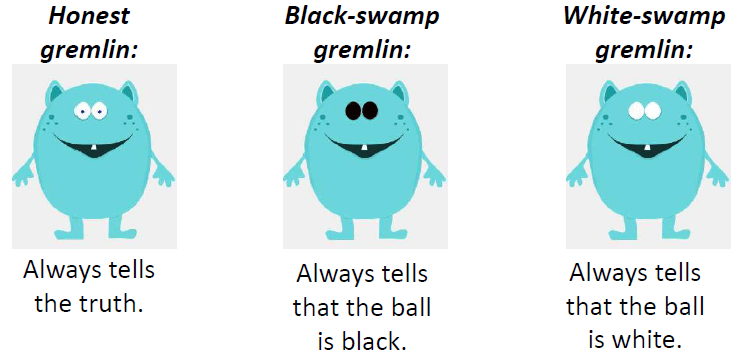
\includegraphics[width=0.6\textwidth]{Graphs/gremlins1.png}
\end{figure}


\bigskip
\noindent\textbf{Belief Elicitation (BE)}.\ \ \ 
As in the IP task, subjects know the prior probability of drawing a black ball and the composition of the group of gremlin providing hints. Instead of making a protection decision, however, subjects are asked to estimate the probability that: (i) the ball is black when the gremlin says that it is white; (ii) the ball is black when the gremlin says that it is black. 

To elicit incentive-compatible responses, we follow the stochastic version of the Becker-DeGroot-Marshak mechanism developed by \citet{grether_testing_1992} and \citet{holt_update_2009} but stated equivalently in terms of losses rather than gains.
 %to match the description of other tasks. 
Subjects submit their beliefs about the probability of the adverse event $\mu \in [0,1]$. If $\mu$ is above some uniform random number $r\in[0,1]$, they lose \$20 only if this event happens (i.e., a black ball is drawn). If $r > \mu$, then they draw an independent lottery that will lose \$20 with probability $r$ and 0 otherwise.\footnote{The benefit of this mechanism versus other probability elicitation mechanisms (e.g., quadratic scoring) is that reporting truthfully is a dominant strategy regardless of risk preferences \citep{karni_mechanism_2009-1} as long as a subject's preferences adhere to probabilistic sophistication and dominance: they rank lotteries based on their probabilities only and prefer higher probabilities of higher payoffs.} Motivated by \citet{danz_belief_2020}, who find that providing a detailed explanation of payoffs can lower truthful reporting, we instead explain that reporting true belief $\mu$ maximizes their payoffs, and give an example of payoff calculation under different reporting strategies.

\bigskip
\noindent\textbf{Willingness to Pay Elicitation (WTPE)}.\ \ \ The WTPE task measures a subject's willingness to pay (WTP) for a signal. As before, subjects know the prior probability of drawing a black ball and the composition of the group of gremlin providing hints.  Unlike the IP task, subjects do not automatically receive a hint, instead they provide their WTP for a hint by choosing a value $\in {\$0,\$5}$ in \$0.50 increments. The elicitation is incentive compatible: if a WTPE round is selected as the payment round, a random price of a hint will be drawn. If that price exceeded the subject's WTP, they will play a BP round, otherwise the subject pays their WTP and plays an IP round.  

\vspace{10pt} 

After the WTPE task, subjects answered a few demographic questions: gender, age, and number of statistics courses they have taken. The payment task and the payment round were then randomly chosen to calculate the subject's payoff. 

For tasks other than BP, subjects go through two different priors and three types of signals. The order is such that subjects go consecutively over all three signal types starting from the honest one for each prior. The order of priors and signals stays constant for each subjects across tasks, but can vary between subjects. Table~\ref{tab:treatments} summarizes our treatments.

%%%%%%%%%%%%%%%%%%%%%%%%%%%%%%%%%%%%%%%%%%%%%%%%%%%%%%%%%%%%%%%%%%%%%%%%%%%%%%%%%%%%%%%%%%%%%%%%%%%%%%%%
\begin{table}[h!]
\caption{List of Treatments} \label{tab:treatments}
\begin{tabular}{l*{6}{c}}
\hline\hline
 & \multicolumn{3}{c} {Gremlins composition} & & \\
Prop. of black balls ($p$) & Honest & Black-eyed &White-eyed & FP rate &  FN rate\\
\hline
0.1, 0.2, 0.3, 0.5         &    2 & 0  &  0 & 0 & 0\\

0.1, 0.2, 0.3, 0.5         &    3 & 1  &  0 & 0.33 & 0  \\

0.1, 0.2, 0.3, 0.5          &    3 & 0  &  1 & 0 & 0.33 \\

0.1, 0.2, 0.3, 0.5           &    3 & 1  & 1 & 0.33 & 0.33\\

0.1, 0.2, 0.3, 0.5         &    5 & 1  & 0 & 0.2 & 0\\
0.1, 0.2, 0.3, 0.5         &    5 & 0  & 1 & 0 & 0.2    \\
0.1, 0.2, 0.3, 0.5         &    5 & 1 & 1  & 0.2 & 0.2  \\
\hline\hline
\end{tabular}


\end{table}

%%%%%%%%%%%%%%%%%%%%%%%%%%%%%%%%%%%%%%%%%%%%%%%%%%%%%%%%%%%%%%%%%%%%%%%%%%%%%%%%%%%%%%%%%%%%%%%%%%%%%%%%

 


\vspace{20pt}
\section{Subject Decisions By Task}\label{sec:sanity}

Decisions in the Blind Protection (BP), Informed Protection (IP), and Belief Elicitation (BE) tasks measure determinants of WTP in our model. Protection choices in the BP task reveals subjects' risk preferences with known probabilities. Choices in the IP task demonstrate how subjects use signals given their characteristics. Finally, the BE task provides insight into subjects' beliefs for given signals.  We briefly discuss patterns of subject decisions below. They suggest that subjects understand these tasks reasonably well.
%Some of these tasks can be quite challenging. However, we show below that 

\subsection{Blind Protection}

Figure~\ref{fig:ProtResponse} plots the likelihood (in blue) of protecting against the posterior probability of a drawing a black ball for the BP task, where the posterior is equivalent to the prior, and in the IP task. On aggregate in the BP task, subjects' likelihood of protecting increases in the probability of a negative outcome: only 13\% subjects protect when the probability of a black ball is 10\% in contrast to 70\% protecting when the probability is 30\%. 

At the individual level, BP responses indicate significant heterogeneity in risk preferences. For approximately 70\% of subjects (72/105), protection action increases monotonically in probability. The remaining 30\% make at least one switch from protecting to not protecting and back, which is inconsistent with EU maximization.\footnote{That is, subjects do not protect for some treatments with posterior probability $P$ while protecting for a posterior probability $P'<P$.  Inconsistency on risk preference measures is well known.  \citet{filippin_reconsideration_2016} found that 17.1\% of more than 6,300 subjects in 54 published papers made inconsistent switches on the Holt and Laury (2002) on paired-lottery measure where options are presented in increasing payoff order, which they are not here. Among these switchers, however, 83\% (24/39) skip only a single increment of the presented probability scale, suggesting an inattention error.}

%\footnote{For comparison, Holt and Laury (2002) for a similar instrument find that 28 of 212 subjects (13\%) switched back to a low-risk option with an increasing likelihood of high payoffs in a risky option at least once when decisions were presented in increasing order, which they are not here.}

Risk-neutral agents who maximize their expected utility should start protecting when the prior exceeds 0.25, i.e., at the ratio of the protection cost to the potential loss = \$5/\$20. Many of our subjects (24) start protecting at lower priors (0.05-0.15), indicating strict risk aversion.  A smaller group of subjects makes choices consistent with risk loving by protecting at a probability of 0.3 or never.\footnote{As a reference using a CRRA utility function, switching at the probability 0.1 corresponds to a coefficient of relative risk aversion $\theta=2$, switching at 0.2 corresponds to $\theta=0.57$, and switching at 0.3 corresponds to $\theta=-0.54$.} 

%\footnote{That is, subjects do not protect for some treatments with posterior probability $P$ while protecting for a posterior probability $P'<P$.}

\subsection{Informed Protection}

Recall that, in the IP task, subjects not only know the prior but also receive a signal (hint) about the ball color. 
Figure~\ref{fig:ProtResponse} shows that protection actions are increasing in the posterior probability of an adverse event, though roughly 28\% of subjects break monotonicity in their protection responses with respect to posterior probabilities --- approximately the percentage of non-monotonic responses in the BP task.  Breaking monotonicity here is not particularly surprising as subjects are not directly given their posterior probabilities and may estimate them incorrectly. At the individual level, we also find that the total number of times subjects protect in the BP task significantly correlates with their likelihood of protection in the IP task conditional on posteriors, but this explains only a very small part ($<$1\%) of variation in the IP decisions.\footnote{We use a linear probability model to estimate this relationship, and while the coefficient on the total number of protection choices is significant at the 1\% level, the $R^2$ only increases from 0.295 to 0.3.} 


%%%%%%%%%%%%%%%%%%%%%%%%%%%%%%%%%%%%%%%%%%%%%%%%%%%%%%%%%%%%%%%%%%%%%%%%%%%%%%%%%%%%%%%%%%%%%%%%%%%%%%%%%%%%%%%%%%%
\begin{figure}[H]
\centering
\caption{Average Protection Response} \label{fig:ProtResponse}
  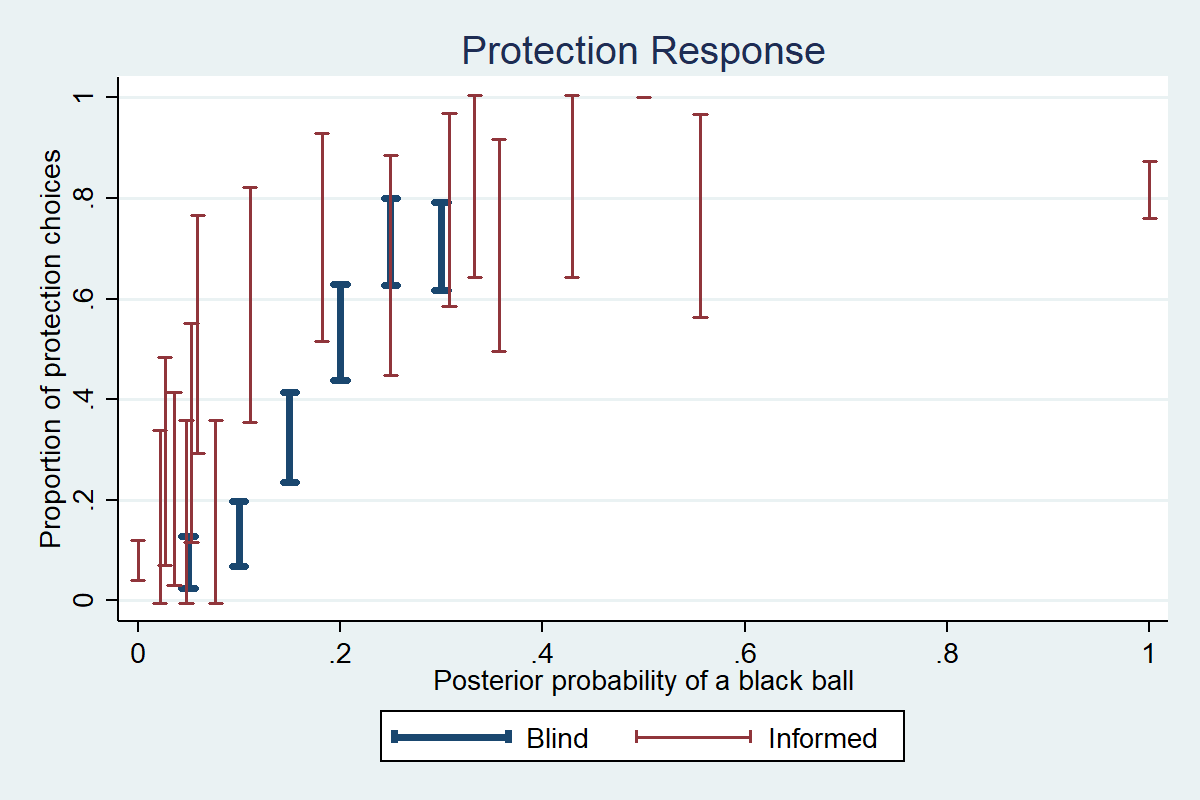
\includegraphics[width=0.7\textwidth]{Graphs/ip_response_comp.png}
\fnote{The bars show 95\% confidence intervals for the mean proportion of subjects choosing protection at each posterior probability.}
\end{figure}
%%%%%%%%%%%%%%%%%%%%%%%%%%%%%%%%%%%%%%%%%%%%%%%%%%%%%%%%%%%%%%%%%%%%%%%%%%%%%%%%%%%%%%%%%%%%%%%%%%%%%%%%%%%%%%%%%%%

Table~\ref{tab:nonparIP} presents the average protection decisions by prior and signal type. The first three columns indicate the signal's characteristics and its realization (hint). Column 4 shows the posterior probability of a black ball averaged across all the treatments within a group, column 5 the subjects' share of empirical protection responses, while column 6 presents the theoretical optimum for a risk-neutral decision maker. Finally, column 7 presents the $p$-value for a test of equality between empirical and theoretical protection responses.

Three observations emerge from the table. First, regardless of the signal's FP and FN rates, black hints substantially increase the likelihood of protection.  Second, subjects' protection decisions deviate significantly from what is optimal for risk-neutral subjects in most treatments, as evidenced by column 7. Subjects significantly overprotect when facing white hints (rows 1--4), while signficantly underprotecting when facing black hints without false positives (rows 5--6).  Subjects overprotect for black hints with false positives, though the difference is not statistically significant. 
%with the exceptions of a black signal from a tester with positive FP rates, where the statistical equality of columns 5 and 6 cannot be rejected (rows 7--8).

%\textbf{In light of BP decisions it is not surprising that subjects do not behave as risk-neutral agents, but some biases cannot be explained by the expected utility maximization for any degree of risk aversion.} 
Third, we find that some deviations cannot be explained by the expected utility maximization for any degree of risk aversion. For example, consider rows 1 and 3: even though an increase in the FP rate does not change the posterior (because the hint is white), the protection rate increases by 6 percentage points (pp)\footnote{The difference is significant at 5\%}. Similarly, comparing rows 3 and 4, we see that introducing false negatives to a signal that also generates false positives raises the protection rate increases to 56 percent --- even though the average posterior probability given the signal's characteristics is merely 13 percent. As a benchmark, with no signal in the BP task, only 13~(32) percent of subjects choose to protect when the probability is 10~(15) percent. 

%%%%%%%%%%%%%%%%%%%%%%%%%%%%%%%%%%%%%%%%%%%%%%%%%%%%%%%%%%%%%%%%%%%%%%%%%%%%%%%%%%%%%%%%%%%%%

\begin{table}[H]\centering 
\caption{Average Protection by Signal Type} 
\label{tab:nonparIP}
\adjustbox{max width=\textwidth}{
	\begin{threeparttable}
	\begin{tabular}{cccccccc} \hline \hline
	\multirow{4}{6ex}{\centering \textbf{Row}}
			&\multicolumn{2}{c}{\centering \textbf{Signal Characteristics}} &\multirow{3}{12ex}{\centering \textbf{Hint}} 
			& \multirow{3}{10ex}{\centering \textbf{Posterior}} & \multirow{3}{10ex}{\centering \textbf{Share Protect}} 
			& \multirow{3}{10ex}{\centering \textbf{Share Optimal}} 
			& \multirow{3}{13ex}{\centering \textbf{P-val $(H_0: (5)=(6))$}} \\ 
			\cmidrule(lr){2-3}
		& \multirow{2}{12ex}{\centering \textbf{False Positive}} 
			& \multirow{2}{12ex}{\centering \textbf{False Negative}} 
		\\
		\\
		&(1) & (2) & (3) & (4) & (5) & (6) & (7) \\
		\hline
			(1)&No&No  &White&0.000&0.067&0.000&0.000\\
(2)&No&Yes &White&0.100&0.333&0.000&0.000\\
(3)&Yes&No &White&0.000&0.130&0.000&0.000\\
(4)&Yes&Yes&White&0.131&0.564&0.121&0.000\\
(5)&No&No  &Black&1.000&0.846&1.000&0.000\\
(6)&No&Yes &Black&1.000&0.841&1.000&0.000\\
(7)&Yes&No &Black&0.550&0.833&0.870&0.355\\
(8)&Yes&Yes&Black&0.483&0.886&0.871&0.685\\

			\\[-1em]
		\hline\hline 
	\end{tabular} 
	\begin{tablenotes}[flushleft]
			\item\leavevmode\kern-\scriptspace\kern-\labelsep \footnotesize \textit{Notes:} 
	\end{tablenotes}								
	\end{threeparttable}
	}
\end{table}



%\bigskip\noindent\textbf{Belief Elicitation.}\ \ \ 
\subsection{Belief Elicitation}
Subject decisions in the IP task capture the use of signals in protection decisions, but decisions reflect but risk preferences and (potentially erroneous) beliefs.  The BP task can be used to construct a measure of the former; the BE task to measure the latter.  


%%%%%%%%%%%%%%%%%%%%%%%%%%%%%%%%%%%%%%%%%%%%%%%%%%%%%%%%%%%%%%%%%%%%%%%%%%%%%%%%%%%%%%%%%%%%%%%%%%%%%%%%%%%%%%%%%%%

\begin{figure}[H]
	\centering
	\caption{Errors in Bayesian Updating} \label{fig:BeliefUpdate}
	\subcaptionbox{Error Distribution}{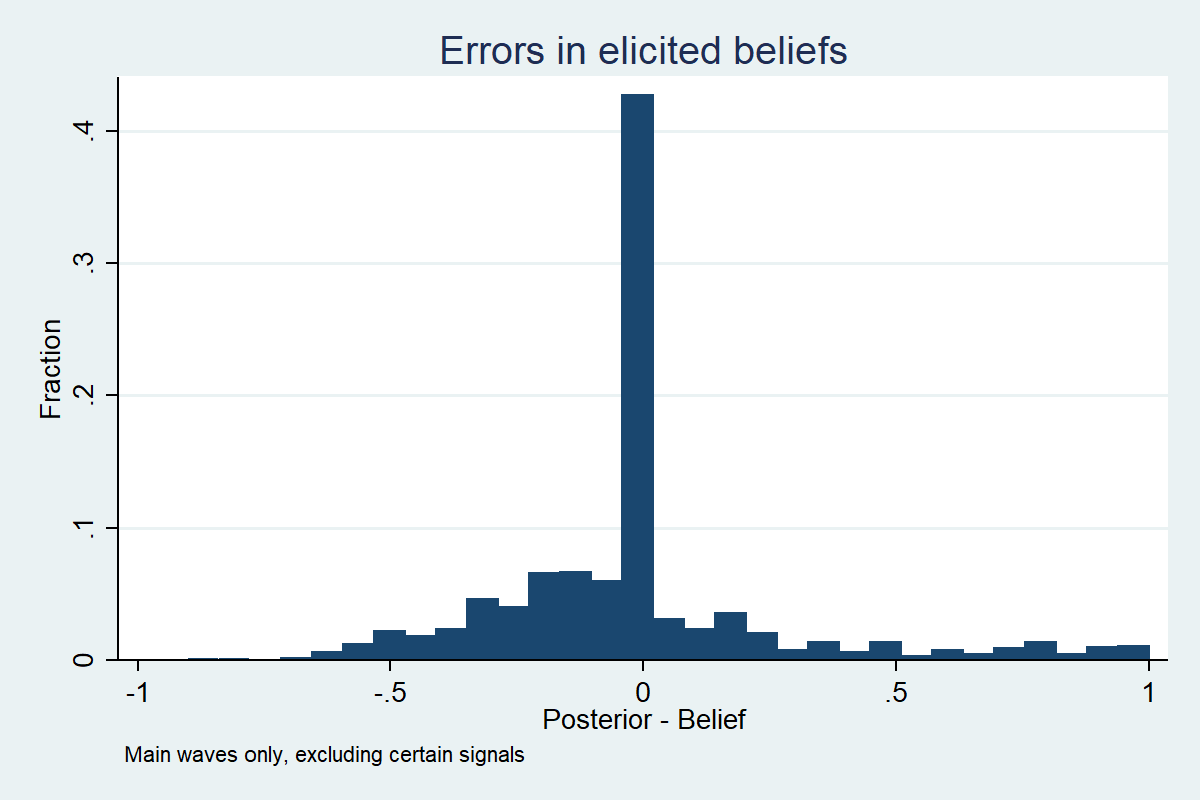
\includegraphics[width=.48\textwidth]{Graphs/hist_belief_error_s3.png}}
	\hfill
	\subcaptionbox{Error v. Posterior}{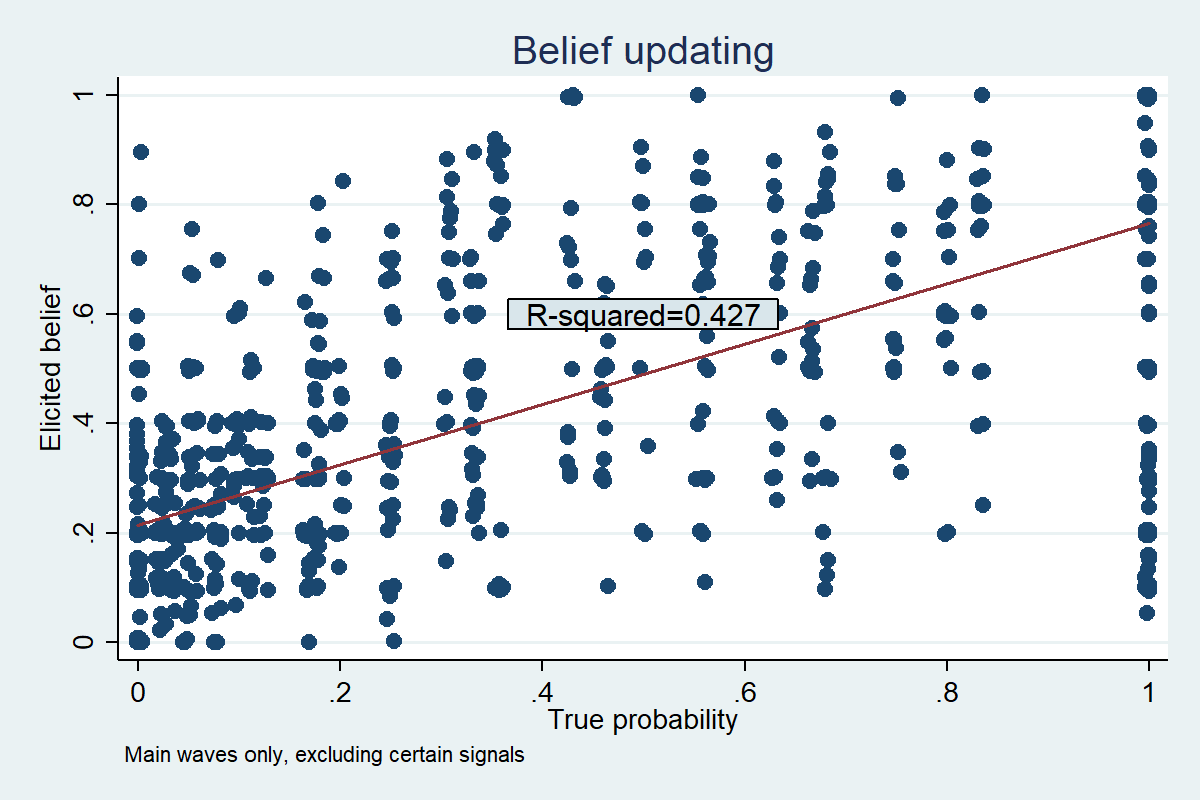
\includegraphics[width=.48\textwidth]{Graphs/updating_s3.png}}
	\hfill
	\vspace{2em}
	\subcaptionbox{Error Distribution, Certain Posterior}{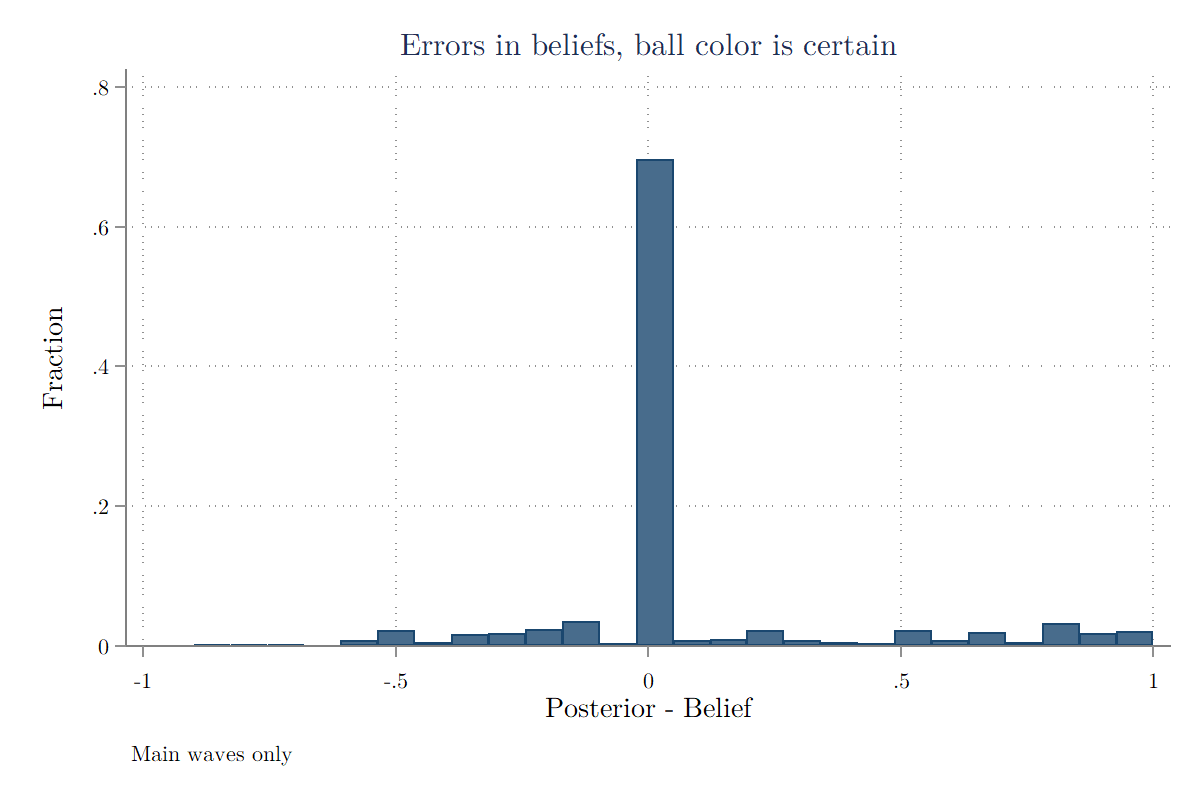
\includegraphics[width=.48\textwidth]{Graphs/hist_belief_error_s5.png}}
	\hfill
	\subcaptionbox{Error v. Posterior, Certain Posterior}{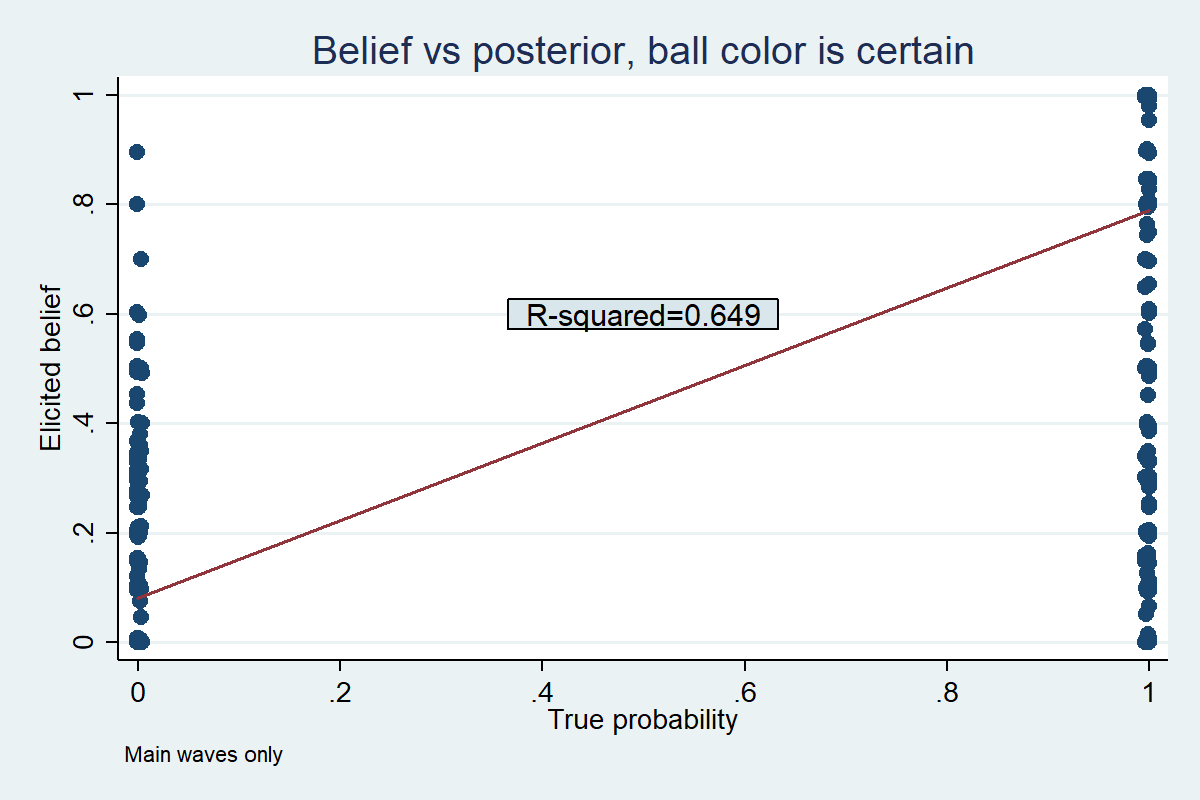
\includegraphics[width=.48\textwidth]{Graphs/updating_s5.png}}
	\hfill
	\vspace{2em}
	\subcaptionbox{Error Distribution, Uncertain Posterior}{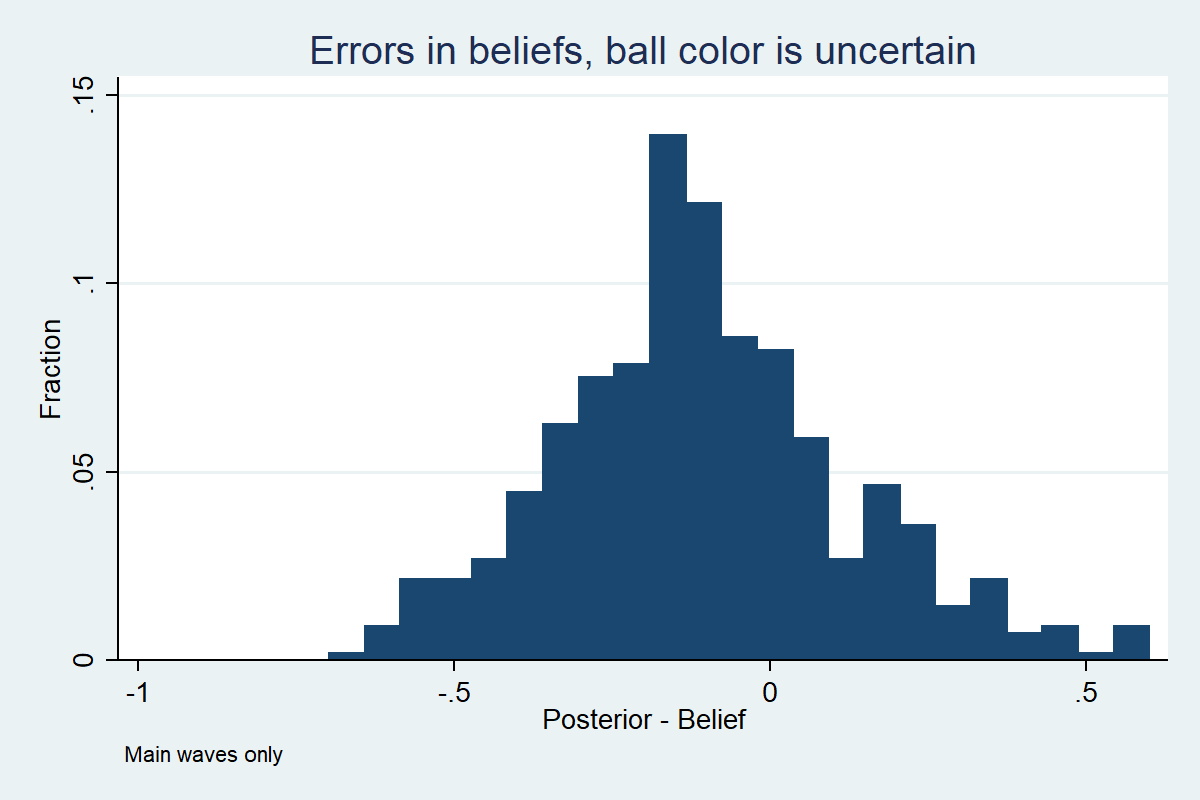
\includegraphics[width=.48\textwidth]{Graphs/hist_belief_error_s4.png}}
	\hfill
	\subcaptionbox{Error v. Posterior, Uncertain Posterior}{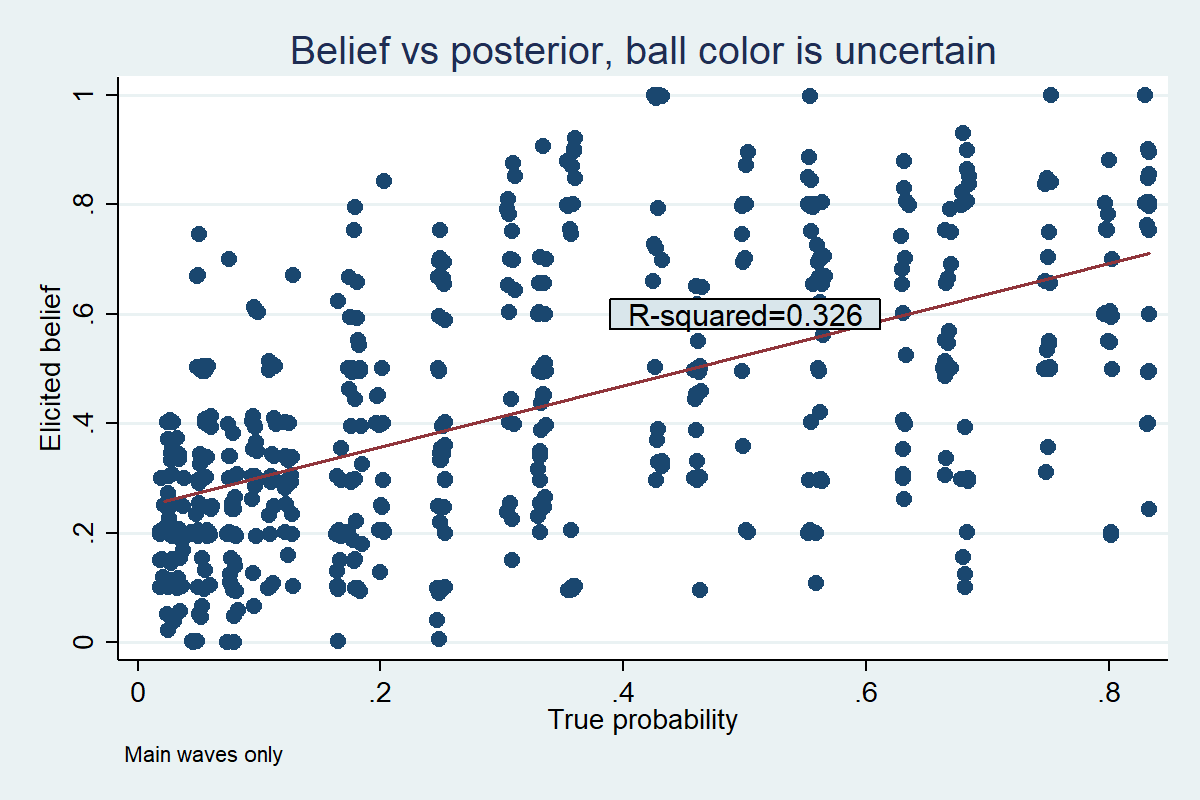
\includegraphics[width=.48\textwidth]{Graphs/updating_s4.png}}
	\hfill
\end{figure}
%%%%%%%%%%%%%%%%%%%%%%%%%%%%%%%%%%%%%%%%%%%%%%%%%%%%%%%%%%%%%%%%%%%%%%%%%%%%%%%%%%%%%%%%%%%%%%%%%%%%%%%%%%%%%%%%%%%

We define updating errors as the difference between the subjects' elicited belief and the actual posterior probability of drawing a black ball for a given signal.  The left-hand column of Figure~\ref{fig:BeliefUpdate} shows the distribution of the updating errors, while its right-hand column presents a scatter plot of the elicited beliefs against the true posterior with a fitted line.
%Since subjects were only given signal characteristics and not true posteriors, their IP responses reflect, inter alia, their ability to infer the true posteriors from signal characteristics. (I'm not sure I like my sentence better)
Panel A uses all observations and suggests that, while errors occur, beliefs are still sensible. The distribution of updating errors is centered at 0, with roughly one-half (51\%) concentrated within +/- 0.1 interval around zero. Overall, the correlation between the elicited beliefs and the true posteriors was 0.653.  

For some combinations of priors and signals, updating should be trivial and posteriors are completely certain.  
%Panel B includes only the 44\% beliefs elicited for an uncertain posterior. 
Panel~B plots such cases, which account for 56\% of the sample and include: (i) treatments with all-honest gremlins; and (ii) treatments with obviously irrelevant dishonest gremlins (e.g., a group gremlins comprising honest and white-swamp gremlins announcing that the ball is black --- or vice versa). Reassuringly, 69\% of reported beliefs are correct. About half of the errors involve reporting a probability of one when it should have been zero.

Meanwhile, Panel~C plots the remaining observations (i.e., with uncertain posteriors). The median error in Panel C is -0.12, with with 90\% of errors lying between -0.48 and 0.3, suggesting that, on average, subjects overestimate the likelihood of adverse events for uncertain posteriors. The correlation between beliefs and posteriors in this sub-sample falls to 0.571.\footnote{The overall pattern of belief updating is consistent with the existing literature which shows that despite updating in the correct direction, people tend to underreact both to the priors and to the signals. The effect of underweighting priors --- first noted in the psychology literature \citep*{phillips_conservatism_1966-1, tversky_belief_1971, kahneman_subjective_1972} --- is known as \emph{representativeness bias} or \emph{base-rate neglect}. Using the regression approach of \citet{grether_bayes_1980}, we find both base-rate neglect and signal underweighting. Our estimates of these parameters are significantly below one with $\hat \alpha=0.43$ $\hat \beta=0.25$ (see Column 1 in \ref{belief_decomposition}). These values are within the range found by the meta-analysis of \citet{benjamin_chapter_2019} which calculates the average $\hat \alpha$ estimate to be around 0.22 (0.4 for incentivized studies only) and the average $\hat \beta$ to be 0.6 (0.43 for incentivized) for studies (like ours) that presented their signals simultaneously.  Such experiments are known as \emph{bookbag-and-poker-chip} experiments} 

%%%%%%%%%%%%%%%%%%%%%%%%%%%%%%%%%%%%%%%%%%%%%%%%%%%%%%%%%%%%%%%%%%%%%%%%%%%%%%%%%%%%%%%%%%%%%

\begin{table}[H]\centering 
\caption{Average Updating Error by Signal Type} 
\label{tab:nonparError}
\adjustbox{max width=\textwidth}{
	\begin{threeparttable}
	\begin{tabular}{ccccccc} 
	\hline \hline
		\multirow{4}{6ex}{\centering \textbf{Row}}
			&\multicolumn{2}{c}{\centering \textbf{Signal Characteristics}} &\multirow{3}{12ex}{\centering \textbf{Hint}} 
			& \multirow{3}{10ex}{\centering \textbf{Posterior}} 
			& \multirow{3}{12ex}{\centering \textbf{Updating Error$^*$}} & \multirow{3}{12ex}{\centering \textbf{P-val $(H_0: Error = 0)$}}  \\ \cmidrule(lr){2-3}
		& \multirow{2}{10ex}{\centering \textbf{False Positive}} & \multirow{2}{12ex}{\centering \textbf{False Negative}} 
		\\
		\\
		& (1) & (2) & (3) & (4) & (5) \\
	
		\hline	
(1)&No&No&White&0.000&0.050&0.000\\
(3)&No&Yes&White&0.100&0.122&0.000\\
(5)&Yes&No&White&0.000&0.122&0.000\\
(7)&Yes&Yes&White&0.131&0.218&0.000\\
(2)&No&No&Black&1.000&-0.163&0.000\\
(4)&No&Yes&Black&1.000&-0.279&0.000\\
(6)&Yes&No&Black&0.550&0.039&0.130\\
(8)&Yes&Yes&Black&0.483&0.048&0.021\\

\\ 	[-1em]
\hline\hline
\end{tabular} 
	\begin{tablenotes}[flushleft]
			\item\leavevmode\kern-\scriptspace\kern-\labelsep \footnotesize \textit{Notes:} $^* \text{Updating error} = Belief - Posterior$. 
	\end{tablenotes}								
	\end{threeparttable}
	}
\end{table}
%%%%%%%%%%%%%%%%%%%%%%%%%%%%%%%%%%%%%%%%%%%%%%%%%%%%%%%%%%%%%%%%%%%%%%%%%%%%%%%%%%%%%%%%%%%%%



Table~\ref{tab:nonparError} summarizes how updating errors vary with the signal's characteristics. We find that subjects overestimate the probability of a black ball when receiving a white hint. This upward bias for a white hint increases in both the FP and FN rates of the signal. To illustrate, consider the change between rows 1 and 3, where introducing a FP rate would not change the posterior because the signal realization is white. Yet, subjects update their posterior upward, magnifying their updating error; we find a similar effect for the introduction of the FN rate (row 1 vs. 2).

The updating bias for black signal realizations (hints), however, varies by information structure. Subjects slightly underestimate the probability with a perfectly accurate signal, but introducing FN rates exacerbates subjects' underestimation. Rows 5 and 6 suggest that the introduction of a FN rate without changing the posterior further reduces subjects' beliefs. With non-zero FP rate, subjects again overestimate the probability of a black ball. The difference in the updating errors for black hints coming from FP-only (row 7) v. FP-FN signals (row 8) is negligible. 
The magnitude of subjects' adjustments to their beliefs was smaller than the actual change to the posteriors due to the FP rates.


\vspace{20pt}

\section{WTP and Signal Characteristics}\label{sec:results}

\subsection{Are Subjects Risk Neutral, Expected Utility Maximizers?} 

\begin{hypothesis}\label{hyp:eqRN} 
Subjects' WTPs for signals are equal to their value for risk-neutral agents. 
\end{hypothesis}

\begin{result} 
On average, there are no significant discrepancies between WTP and predicted value for risk-neutral agents. When splitting by a signal type, a difference emerges only for signals with both false-positive and false-negative rates.
\end{result}



%The model provides a simple benchmark to evaluate potential welfare gains from the signal. Depending on the assumptions on signal characteristics and risk preferences, agents can pay more or less than the risk-neutral benchmark.
%
%We next examine whether subjects understand the WTPE task. One of the model's basic prediction is that signal value decreases with false positive and false negative rates. If subjects understand the basic premise of the WTPE, then we expect a negative correlation between the WTP and the signal's false positive and false negative rate. 

Overall, the theoretical signal's value for a utility maximizing risk-neutral subject (hereafter, the risk-neutral WTP) in equation~\ref{eq:rnWTP} is a useful benchmark of our subjects' WTP. Figure~\ref{fig:WTPhist} plots the distribution of the differences between subjects' WTP and this value.  
%WTP is bounded between \$0 and \$5, where the latter is because protection can be purchased for \$5 so if information were that valuable, an individual would just choose to protect.  
The distribution is centered around 0, indicating that average choices do not fall far from the choices of a risk-neutral utility maximizer. However, there is substantial variation: only 25\% of reported WTP are within \$0.50 of the risk-neutral signal value, and subjects overvalue signals by at least \$1.5 in 22\% of cases and undervalue by at least \$1.5 in 19\% of cases. Introducing FP and FN rates does not increase the range or variation of discrepancies, but introduces a long tail of positive discrepancies shifting the average upward.


\begin{figure}[H]\centering 
	\caption{Discrepancy (Observed WTP - Signal value) by Signal Type} \label{fig:WTPhist}
	\subcaptionbox{All signals}{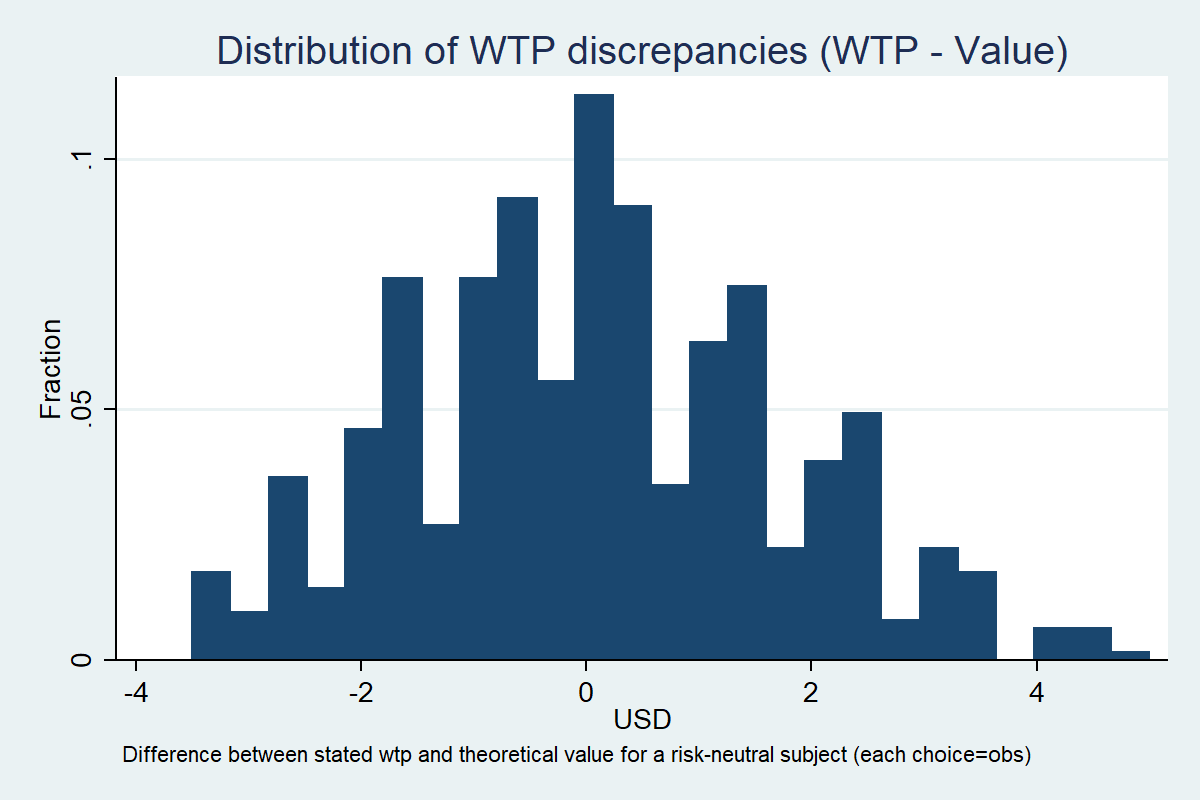
\includegraphics[width=.48\textwidth]{Graphs/hist_WTP_discr1.png}}
	\hfill
	\subcaptionbox{FP only}{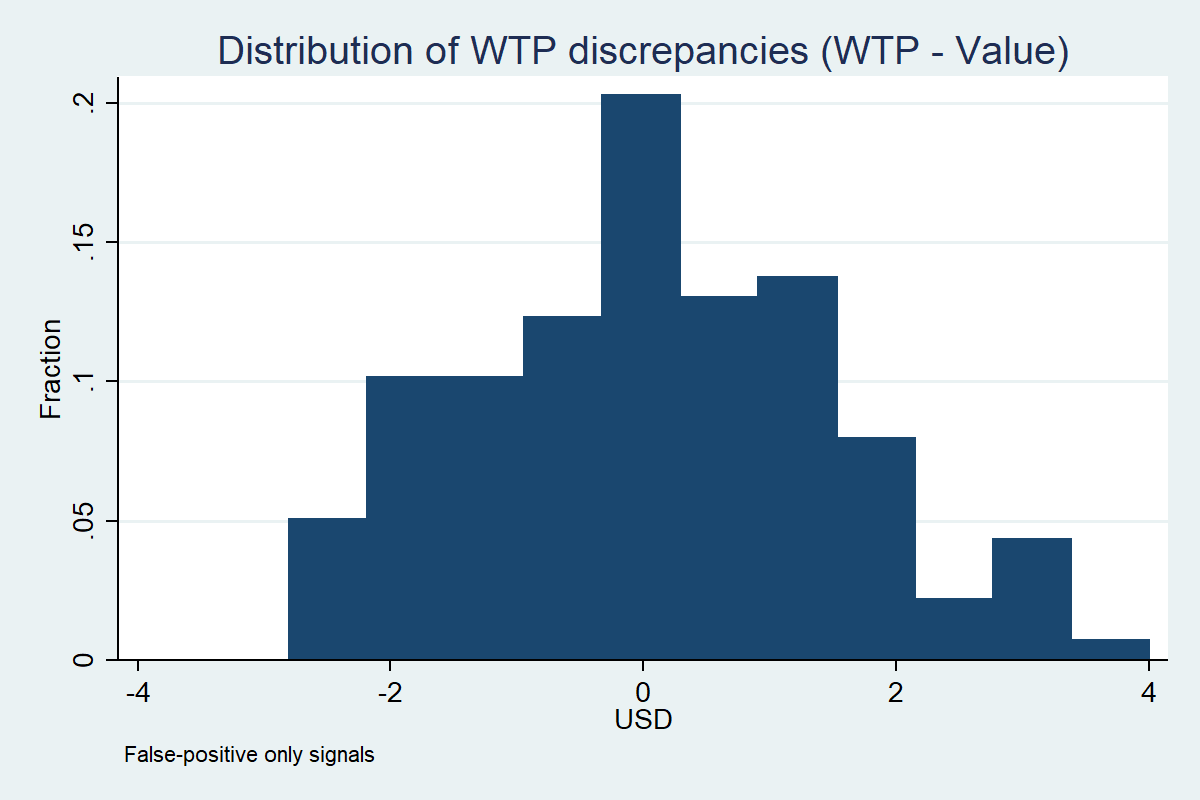
\includegraphics[width=.48\textwidth]{Graphs/hist_WTP_discr1fp.png}}
	\hfill
	\vspace{2em}
	\subcaptionbox{FN only}{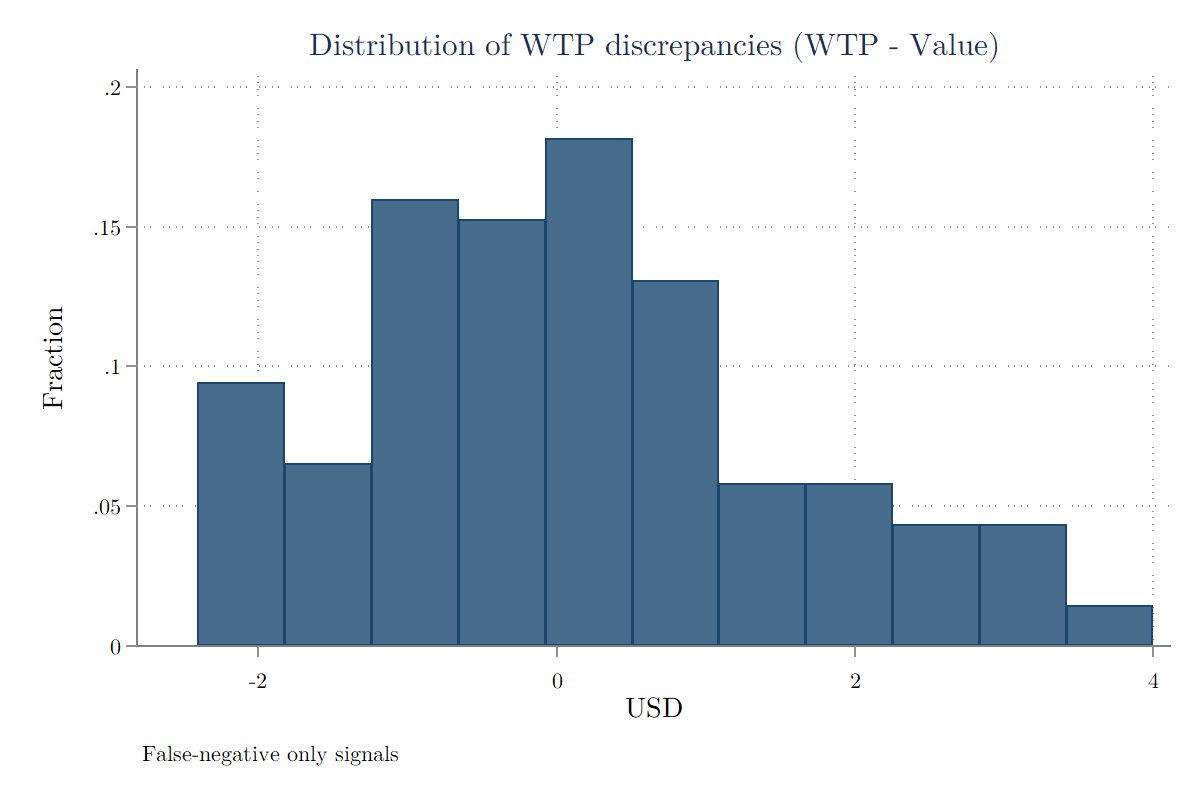
\includegraphics[width=.48\textwidth]{Graphs/hist_WTP_discr1fn.png}}
	\hfill
	\subcaptionbox{Both FP and FN}{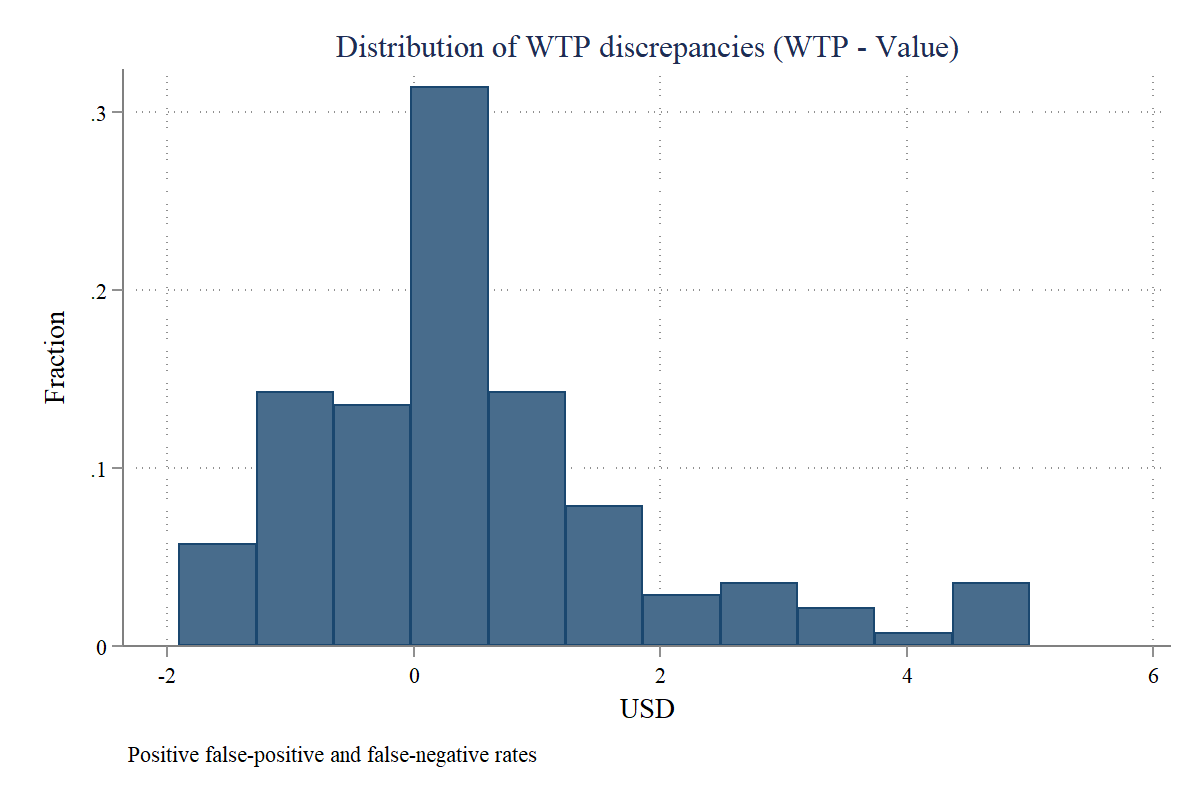
\includegraphics[width=.48\textwidth]{Graphs/hist_WTP_discr1fpfn.png}}
	\hfill

\end{figure}

Our non-parametric analysis in Table~\ref{tab:WTP_nonpar} also finds no differences on average between the observed WTP and the risk-neutral WTP for 3 out of 4 signal's types: honest (i.e., perfectly accurate), FP-only, and FN-only. With both FP and FN rates, however, subjects' WTPs are significantly higher than the risk-neutral WTP. Subjects' overvaluations were similar for both low and high priors. Note, that these signal characteristics induce overprotection in the IP task. Subjects tend to overpay for signals with positive FP rates when the prior is low (0.1 or 0.2), and for signals with positive FN rates when the prior is high (0.3 or 0.5).


%%%%%%%%%%%%%%%%%%%%%%%%%%%%%%%%%%%%%%%%%%%%%%%%%%%%%%%%%%%%%%%%%%%%%%%%%%%%%%%%%%%%%%%%%%%%%%%%%

%\begin{table}[H]\centering \caption{Average WTP discrepancy (WTP-Value) by Signal Type} \label{WTP_nonpar} \begin{tabular}{cccc} \hline \hline
\multirow{2}{12ex}{\centering \textbf{False positive}}&\multirow{2}{12ex}{\centering \textbf{False negative}}&\multirow{2}{15ex}{\textbf{\centering Mean WTP discrepancy}}& \multirow{2}{10ex}{\centering \textbf{P($=0$)}}\\ 
\\
\hline
No&No&-0.106&0.433\\
No&Yes&0.143&0.250\\
Yes&No&0.081&0.502\\
Yes&Yes&0.492&0.000\\
\hline \end{tabular} \end{table}


\begin{table}[H]\centering \caption{Average WTP discrepancy (WTP-Value) by Signal Type} \begin{tabular}{ccccc} \hline \hline
\textbf{Priors}&\textbf{Honest}&\textbf{FN only}& \textbf{FP only} & \textbf{FP and FN}\\ \hline
All priors&-0.106&0.143&0.081&0.492***\\
Low priors&-0.135&-0.209&0.465**&0.437**\\
High priors ($>$0.2)&-0.077&0.496*&-0.303&0.547**\\
\hline \\ \end{tabular} \end{table}


%To understand how subjects' WTP deviates from these risk-neutral signal value, we use a regression analysis of discrepancies between reported WTP and theoretical values to understand, first, the validity of a risk-neutral model and, second, relative weights put on false-negative and false-positive costs. 



\begin{hypothesis}\label{hyp:eqSen} 
Subjects' preferences demonstrate equal sensitivity to costs generated by false-positive and false-negative events. 
\end{hypothesis}

\begin{result} 
On average for our signal and sample structure, we cannot reject the hypothesis of equal sensitivity. However, we observe significant heterogeneity with respect to priors: subjects tend to overvalue false-negative costs for low probability events and overvalue false-positive costs for high probability events. 
\end{result}


In order to examine how WTP responds to signal's quality. We estimate the relationship between WTP biases and signal characteristics with the following regression:
\[\Delta b_{is} = \beta_0 + \beta_1 FP + \beta_2 FN + \varepsilon_{is}\]
where $\Delta b_{is} = (b_{is} - b^*_s)$ is the difference between the WTP of individual $i$ for signal $s$ and $b^*_s$ is the risk-neutral WTP; FP (FN) is the false positive (false negative) cost.  It is worth reiterating at this point that false positive or false negative \textit{costs} are functions of both the rates and the costs of the consequences of those rates.  For example, a high false-negative rate imposes fewer costs when priors are low because the adverse outcome is already unlikely, whereas high false-negative rates carry substantial costs when the prior probability of the adverse outcome is high. All specifications include subject fixed effects, with standard errors clustered at the subject level. If subjects are risk-neutral expected-utility-maximizers, we expect $\beta_1=0$ and $\beta_2=0$. The result, reported in column 1 of Table~\ref{tab:wtp_ols}, shows positive and statistically significant coefficients for both FP and FN costs with highly significant model's F-test. In other words, subjects deviate by overpaying for inaccurate signals. 


%\subsection{The (As-)symetry of False Positive and False Negative Signals} 

%First, subjects' WTPs for a signal are equal to its value for risk-neutral agents. The model provides a simple benchmark to evaluate potential welfare gains from the signal. Depending on the assumptions on signal characteristics and risk preferences, agents can pay more or less than the risk-neutral benchmark.
%
%Second, subjects' preferences value the marginal costs from false-negative and false-positive information equally. The model of a risk-neutral agent suggests that they should. Our derivations above indicate that the relative weight of false-negative costs can be either below or above one depending on risk preferences only.

%\begin{hypothesis}\label{hyp:eqRN} 
%Subjects' WTPs for a signal are equal to its value for risk-neutral agents. 
%\end{hypothesis}

%%%%%%%%%%%%%%%%%%%%%%%%%%%%%%%%%%%%%%%%%%%%%%%%%%%%%%%%%%%%%%%%%%%%%%%%%%%%%%%%%%%%%%%%%%%%%%%%%


\begin{table}[htbp!]f
\centering
\adjustbox{max width = \textwidth}{
	\begin{threeparttable}
	\caption{Deviations from Signal Value (WTP - Value) and Signal Characteristics}
	\label{tab:wtp_ols}
	\begin{tabular}{l*{5}{c}}
		\hline\hline
		&\multicolumn{3}{c}{\multirow{2}{*}{All}} & \multicolumn{2}{c}{Prior}\\ \cmidrule(lr){5-6}
		&&&& $\{.1,.2\}$ & $\{.3,.5\}$\\ 
		\cmidrule(lr){2-4} \cmidrule(lr){5-5} \cmidrule(lr){6-6}  
		&\multirow{1}{*}{(1)} & \multirow{1}{*}{(2)} & \multirow{1}{*}{(3)} & \multirow{1}{*}{(4)} & \multirow{1}{*}{(5)}\\
	\hline
	\\ [-0.5em]
		\exInput{Tables/wtpdiff_ols.tex}
				\hline
		Subject FE & Yes & Yes & Yes & Yes & Yes \\
		Inaccurate Belief Interactions & No & No & Yes & Yes & Yes \\
		Prior Probability FE & No & No & No & Yes & Yes \\
		\hline\hline
	\end{tabular}
	\begin{tablenotes}[flushleft]
		\item\leavevmode\kern-\scriptspace\kern-\labelsep \small\textit{Notes:} Standard errors in parentheses.  In the bottom panels, we also test whether the total coefficient value (baseline+interaction) are different from zero. \sym{*} \(p<0.10\), \sym{**} \(p<0.05\), \sym{***} \(p<0.01\).
	\end{tablenotes}
	\end{threeparttable}
}
\end{table}		
		
%%%%%%%%%%%%%%%%%%%%%%%%%%%%%%%%%%%%%%%%%%%%%%%%%%%%%%%%%%%%%%%%%%%%%%%%%%%%%%%%%%%%%%%%%%%%%%%%%


The risk-neutral model predicts that subjects should value the marginal costs of false-negative and false-positive events symmetrically. Table~\ref{tab:wtp_ols} shows that the coefficient on FN costs is slightly larger indicating higher sensitivity to FP costs, but we cannot reject the hypothesis that the two coefficients are equal. However later we note that this equivalency breaks down when considering specific priors.

\subsection{Risk Preference and Belief Accuracy}

Our baseline estimation in column 1 indicates significant deviations from the model's predictions. Positive and significant coefficients on FP and FN costs indicate that subjects reduce their WTP with growing FP and FN rates by less than a risk-neutral decision-maker would, i.e., subjects' WTP does not respond enough to decreasing quality.

Our benchmark model assumes both perfect updating and risk neutrality, assumptions which open two channels through which deviations could occur. First, Proposition~\ref{thm:riskAverse} suggests that risk preferences can influence the sensitivity of WTP to these signal's characteristics. Second, systematic biases during updating can also lead to deviations. 

We find that risk preferences matter for sensitivity to signal's quality. We use data from the BP task to categorize subjects by their risk preference. We classify all the subjects with internally consistent BP choices into three categories: risk averse, risk neutral, and risk loving.\footnote{We classify subjects based on the total number of protection choices made in the BP task with 2 or 3 choices corresponding to risk-neutrality (protecting starting from 0.2 or 0.25), but exclude subjects making more than one choice at odds with a consistent risk preference.} Column 2 explores the heterogeneity of subject responses to FP and FN costs by their risk preferences, with risk-neutral as the default category. 
%The coefficients for risk-neutral subjects are a bit larger than those of the average subjects (column 1), indicating a higher bias. 
The WTP discrepancies of both risk-neutral and risk-loving subjects increase with FP (statistically insignificant) and FN costs --- suggesting that they did not downward-adjust their WTP enough to account for lower quality signals. In contrast, the WTP discrepancies of risk-averse subjects show hardly any sensitivity to FP and FN costs.  

Accounting both for belief accuracy and risk preferences does little to explain the pattern of underreacting to FP and FN rates. We use data from the BE task to construct a measure of subjects' belief accuracy.\footnote{We calculate a belief error as the absolute value of the difference between the subject's belief and the true posterior probability and then average these errors across all the decisions with identical priors, false positive and false negative rates. A subject's posterior belief for a decision is defined as accurate if its error is less than the median error across all the subjects making the same decision.} Column 3 presents the most flexible specification that controls for belief accuracy and risk preference by including triple interactions of belief accuracy, risk preference, and signal characteristics. The baseline group is the group of risk-neutral subjects with relatively accurate beliefs. We find a lower sensitivity to FP costs for risk-neutral subjects with accurate beliefs and very little change to the corresponding sensitivity to FN costs. This indicates that even relatively accurate Bayesians did not downward-adjust their WTP enough to increasing FP/FN costs.\footnote{Aside from these theoretically motivated individual differences, we investigate several other characteristics.  Heterogeneity is not driven by demographic characteristics (e.g., age, gender) or prior statistical coursework.  These results are in Appendix A Table~\ref{wtp_dem}.}
  

\subsection{Heterogeneity by Prior}

We motivate our experiment with a real-world problem of designing warning systems --- often for events with low probabilities. With a low prior, the default action of risk-neutral subject would be not to protect, and vice versa with a high prior. The signal would help risk-neutral subjects decide whether to keep the default action or to switch. We split the prior by below/above 0.25 (= protection cost/potential loss), and we incorporate prior-probability fixed effects to the aforementioned flexible specification. 

Column 4 of Table~\ref{tab:wtp_ols} presents the results for low-prior WTPE tasks. With low priors, deviations from the risk-neutral WTP increase with FP costs: subjects overvalue signals that would induce them to overprotect. This overvaluation is similar for different risk preference profiles. Column 5 presents the results for high-prior WTPE tasks. With high priors, the deviations of risk-neutral and risk-loving subjects from the risk-neutral WTP increase with FN costs. These subjects did not downward-adjust their WTP enough to account for increasing FN rates and overvalue signals that would induce them to underprotect. 
 %and reduce their WTP less per dollar of expected false-negative costs as indicated by positive and significant coefficient. 
%At the same time, the coefficient on FP costs goes down indicating higher sensitivity to FP costs. Risk-averse subjects even overreact to false-positive cost though the effect is not significant given our sample size. 

In summary, most subjects underreact to false-positive costs with low priors and underreact to false-negative costs for high priors. In practice, and given low priors implied by many alert systems, this means that users would mostly overpay for alert signals with high false-positive costs, while excessively discounting signals with significant false-negative rates. For example, individuals would prefer a smoke alarm that never misses fires even if it involves higher expected costs of false alarms. Risk preferences affect this pattern with risk-averse subjects moving closer to a risk-neutral benchmark, but most interaction coefficients are not statistically significant despite large magnitudes.

%While this finding is incidental and not the part of the original research plan, its significant practical implications prompt us to explore it further.





%\subsection{Discussion: What Accounts for the Heterogeneity by Prior?}
\section{Discussion}

Subjects' underreactions to false-positive (false-negative) costs for low (high) priors present a puzzle. These behaviors are inconsistent with our risk-neutral model: Equations~\ref{eq:dWTP_dFP} and~\ref{eq:dWTP_dFN} suggest that WTP should respond more to FP rates (relative to FN rates) for low priors and vice versa for high priors. As stated earlier, for a given FN rate, false-negative events are much less likely with low priors and hence impose lower costs on the agent. As priors increase, FN rates become more salient while FP rates become less salient. Instead, our subjects react very similarly to FP and FN rates for both low and high priors. The divergence between our subjects' WTP and the risk-neutral WTP explains changing signs on FP and FN costs in the previous regressions of WTP differences.



\begin{figure}[H]
\centering
\caption{Theoretical and Empirical WTP Sensitivities to FP and FN rates} \label{fig:Comparison}
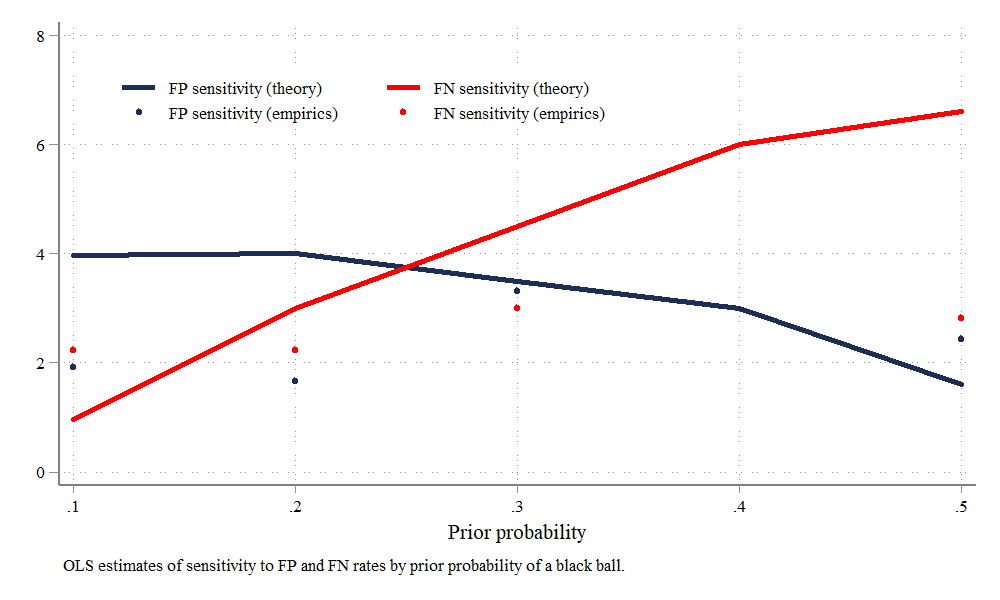
\includegraphics[width=0.8\textwidth]{Graphs/sensit_comparison.png}
\end{figure}

Figure~\ref{fig:Comparison} illustrates this puzzling behavior. This figure plots estimates from the regression of reported WTP --- instead of its deviation from the risk-neutral WTP --- on FP and FN rates. We find that the sensitivities of subjects' WTP to both FP and FN rates increase with priors and that the change occurs relatively smoothly. Two sensitivities are also surprisingly close to each other.\footnote{We cannot reject the hypothesis that two sensitivities are equal to each other for any of the priors.} 

We consider four candidate explanations: risk preferences, anchoring bias, valuing non-instrumental information, and finally a failure to distinguish how FP and FN error rates ought to differently affect calculated posteriors. 

\emph{Risk} Our evidence suggests that risk preference cannot explain this behavior. We test the risk preference hypothesis using subjects' BP choices. Columns 4--5 of Table~\ref{tab:wtp_ols} already show that, even after controlling for subjects' risk preferences, the coefficients on FP and FN costs remain very different for low and high priors.

We augment this analysis in Table~\ref{tab:wtp_risk} (Appendix) by explicitly testing for interactions between risk-preferences, priors, and FP and FN rates. We find that these interactions are mostly insignificant, with the exception of interactions between FN rates and risk aversion for some specifications. The heterogeneity largely remains after controlling for risk preferences, but the interaction between high priors and FP rates becomes insignificant.

\emph{Anchoring} The evidence also does not support the hypothesis that subjects anchored on previous priors. Each subject goes through two sets of treatments with two different priors in a fixed order, so anchoring could occur.  We find, however, that most subjects (92 out of 104) change their decisions when going from one prior to another, and the average belief error in the BE task is actually \emph{lower} for the second set of priors rather than the first, which suggests that changing priors does not make subjects more confused. Most importantly, we cannot see statistically significant differences between FP and FN coefficient estimates even if we limit our attention only to the first priors in each sequence.\footnote{Depending on session, the first 3 WTP treatments use either 0.1 or 0.2 as the prior, so there is no anchoring on the previous prior or something special about a particular prior.}

\emph{Non-instrumental information} There is evidence in the literature of people valuing "non-instrumental information'' that does not affect their decisions. Most information in our experiment is instrumental by design (it helps to choose actions) and indeed enters into subjects' decisions as evidenced by choices in the IP task. Nonetheless, many subjects have a positive WTP for signals that cannot affect their IP decisions (159 out of 624 total choices). It is therefore plausible that the reported WTPs includes some non-instrumental components. 

However, we think that preferences for non-instrumental information cannot provide a full explanation of our results. The main reason is that our experiment has no time delay between receiving a signal and learning the outcome. If the WTP task round is selected as a payment round, the subject receives a signal, chooses an action and then immeditealy learns the experiment's payoffs. Hence, there is practically no window for subjects to experience any anticipatory feelings which the literature assumes to be the standard causal mechanism behind the demand for non-instrumental information. Second, the closeness of coefficients for FP and FN rates also seems apriori implausible based only on the non-instrumental information value story because, in contrast to our next explanation, no theory of preferences for non-instrumental information imposes restrictions on these coefficients.

\emph{Failure to distinguish FP and FN} Instead, we argue that subjects' observed behaviors arise from confusing FN and FP rates. We use as evidence subjects' own proffered explanation.  At the end of the experiment, we asked subjects to explain to us how they made their protection choices.  Out of 105 subjects in the main waves of the experiment, 39 refer to the \textit{percentage} \normalfont  of dishonest gremlins as their rationale for choosing protection. For example:
\begin{itemize}
	\item ``\emph{my strategy for this task was to only buy protection if there was a white or black gremlin and not if there was a truth gremlin}''
	\item ``\emph{If there were only honest gremlins then I never protected but even if there was one white-swamp gremlin or one black-swamp gremlin then I payed for protection.}''
\end{itemize}

Among the other 66 subjects, some may use this heuristic without describing it.\footnote{The text of all responses are in the appendix}  The closeness of the coefficient estimates for FP and FN rates in Table ~\ref{tobit_het} are certainly consistent with these statements. If subjects neglect the difference between FP and FN risks when choosing their WTP, it would explain both the coefficients' similarity and their lack of variation with respect to priors. Indeed, if subjects treat FP and FN rates the same and consider only the total proportion of false signals, they would assign equal weights to each of them, and the best fit line of signal's value with the respect to the sum of FP and FN rates should be relatively flat because priors affect FP and FN costs in opposite ways.\footnote{The equality of coefficients on FP and FN rates is a necessary prediction of this explanation, but can emerge only by chance with (some) heterogeneous risk preferences.}

In order to test this hypothesis, we use choices from the BE and IP tasks where subjects face imperfect signals. If subjects systematically neglect the difference between FP and FN rates, we expect to find the pattern of unexplained reaction to FP and FN rates in cases when they do not affect the posterior. Namely, subjects would show sensitivity to FP rates when the signal is white and sensitivity to FN rates with black (positive) signals. This happens because some subjects react to FP rates as if they are FN rates, and vice-versa. If present, this pattern cannot be explained by any distribution of risk preferences or by anchoring on previous priors.  In Table~\ref{updateErrorReg} we estimate a linear regression of updating error, i.e., actual posterior - reported belief, on FP and FN rates by signal color with individual fixed effects to control for updating biases. Consistent with our conjecture, we observe that the FP rate has a significant positive effect on the error when the signal is white (negative), and that FN rate has a significant negative effect when the signal is black (positive). 



%%%%%%%%%%%%%%%%%%%%%%%%%%%%%%%%%%%%%%%%%%%%%%%%%%%%%%%%%%%%%%%%%%%%%%%%%%%%%%%%%%%%%%%%%%%%%


\begin{table}[htbp]\centering 
\caption{Updating Errors in BE Task} 
\label{updateErrorReg}
\adjustbox{max width=\textwidth}{
	\begin{threeparttable}
	\begin{tabular}{l*{3}{c}}
	\hline\hline
									&\multirow{2}{8ex}{\centering All}&\multicolumn{2}{c}{Signal Received}\\ \cmidrule{3-4}
									&&\multicolumn{1}{c}{White}&\multicolumn{1}{c}{Black}\\
									&\multicolumn{1}{c}{(1)}&\multicolumn{1}{c}{(2)}&\multicolumn{1}{c}{(3)}\\
	\hline

	FP rate         &    0.600\sym{***}&    0.292\sym{***}&    0.908\sym{***}\\
                &  (0.057)         &  (0.063)         &  (0.102)         \\
FN rate         &    0.011         &    0.273\sym{***}&   -0.251\sym{***}\\
                &  (0.053)         &  (0.061)         &  (0.084)         \\
Constant        &   -0.078\sym{***}&    0.314\sym{***}&   -0.470\sym{***}\\
                &  (0.007)         &  (0.009)         &  (0.013)         \\
\hline
Observations    &     1248         &      624         &      624         \\
Adjusted \(R^{2}\)&    0.146         &    0.415         &    0.521         \\

	\\ [-1em]
	\hline
	Subject FE      &      Yes         &      Yes         &      Yes         \\
	\hline
	\hline\hline
	\end{tabular}
	\begin{tablenotes}[flushleft]
			\item\leavevmode\kern-\scriptspace\kern-\labelsep \footnotesize \textit{Notes:} Standard errors in parentheses. \sym{*} \(p<0.10\), \sym{**} \(p<0.05\), \sym{***} \(p<0.01\). 
	\end{tablenotes}								
	\end{threeparttable}
	}
\end{table}


%%%%%%%%%%%%%%%%%%%%%%%%%%%%%%%%%%%%%%%%%%%%%%%%%%%%%%%%%%%%%%%%%%%%%%%%%%%%%%%%%%%%%%%%%%%%%



%%%%%%%%%%%%%%%%%%%%%%%%%%%%%%%%%%%%%%%%%%%%%%%%%%%%%%%%%%%%%%%%%%%%%%%%%%%%%%%%%%%%%%%%%%%%



To further explore this hypothesis, in Table~\ref{tab:protectReg}, we regress IP decisions on FP and FN rates and flexible controls of both posteriors and reported beliefs:\footnote{Given that the true functional form is unknown, we use a linear probability model to get unbiased coefficient estimates.}

	\[Prob(s_{ij}=1)=\alpha_i+\beta_1 P_{10}+\beta_2 P_{01} +Z(P_{ij})+Z(\mu_{ij})+\epsilon_{ij} \]
Here $s_{ij}$ is the protection decision of subject $i$ in treatment $j$, $\alpha_i$ is subject FE, $P_{10}$, $P_{01}$ are FP and FN rates and $Z(P_{ij})$ and $Z(\mu_{ij})$ are the splines of FP/FN rates  and reported beliefs $\mu_{ij}$ to control for these variables in a flexible way. Each spline is a function $Z(x)$ which is just linear $x+C$ within one interval, and constant everywhere else. The splines are constructed so that their linear intervals cover the whole domain of probabilities and beliefs $[0,1]$.\footnote{We use Stata mkspline command to create 5 splines $z_1(x),z_2(x),..z_5(x)$ of initial variable $x$ over the range $[0,1]$ such that $z_k(x)=\min[0,x-x_{k-1},x_k-x_{k-1}]$ with $x_k$ being equally spaced knot values. Splines account for potential nonlinear effects of posteriors and beliefs on protection decision with limited effect on degrees of freedom.} Columns 1 and 2 include only the flexible controls of the true posteriors. Columns 3 and 4 add further flexible controls to account for subjects' (often incorrect) beliefs, inferred from their BE responses.

Columns 1 and 2 show that, even conditional on posterior and subject FEs that account for risk preferences, IP responses are still affected by FP and FN rates. For a white hint, FP and FN rates increase the tendency to overprotect while the FP rate had an opposite effect with comparable magnitude but without statistical significance for a black hint. Hence the first prediction of a conjecture of indiscriminate FP/FN rate use holds: FP rates increase protection when the signal realization is white conditional on the posterior. The effect holds if allowing for heterogeneity of sensitivities to FP and FN rates with respect to priors (Column 2), though the effect of the FN rate for black hints is small in magnitude and not statistically significant at conventional levels. Adding flexible controls for subjects' beliefs reduces the coefficient magnitude on FP rate for white hints (Columns 3 and 4), but the coefficients still remains significant. This indicates that while beliefs partially contribute to these protection anomalies, they cannot explain them completely.
% (possibly due to subjects re-evaluating their beliefs between tasks). 


%%%%%%%%%%%%%%%%%%%%%%%%%%%%%%%%%%%%%%%%%%%%%%%%%%%%%%%%%%%%%%%%%%%%%%%%%%%%%%%%%%%%%%%%%%%%%
\begin{table}[htbp]\centering 
\caption{Informed Protection Response} 
\label{tab:protectReg}
\adjustbox{max width=\textwidth}{
	\begin{threeparttable}	
	\begin{tabular}{l*{4}{c}}
	\hline\hline
									&\multicolumn{1}{c}{(1)}&\multicolumn{1}{c}{(2)}&\multicolumn{1}{c}{(3)}&\multicolumn{1}{c}{(4)}\\
	\hline
		
		FP rate x (S=White)&     .461\sym{***}&     .494\sym{**} &     .282\sym{**} &     .286         \\
                &    (3.3)         &    (2.4)         &    (2.0)         &    (1.4)         \\
FN rate x (S=White)&     .544\sym{***}&     .474\sym{**} &     .195         &     .125         \\
                &    (2.9)         &    (2.1)         &    (1.0)         &    (0.5)         \\

S=Black         &      .42\sym{***}&     .429\sym{***}&     .316\sym{**} &     .336\sym{**} \\
                &    (2.7)         &    (2.7)         &    (2.0)         &    (2.1)         \\
FP rate x (S=Black)&    -.256         &    -.225         &    -.379         &    -.389         \\
                &   (-0.5)         &   (-0.4)         &   (-0.8)         &   (-0.7)         \\
FN rate x (S=Black)&    .0494         &    -.027         &  -.00394         &   -.0879         \\
                &    (0.5)         &   (-0.2)         &   (-0.0)         &   (-0.6)         \\
p$=$0.2         &     .113\sym{***}&     .101\sym{***}&      .09\sym{***}&    .0723\sym{**} \\
                &    (4.2)         &    (2.8)         &    (3.6)         &    (2.1)         \\
FP rate x (p=0.2)&                  &   -.0363         &                  &   .00218         \\
                &                  &   (-0.2)         &                  &    (0.0)         \\
FN rate x (p=0.2)&                  &     .122         &                  &     .127         \\
                &                  &    (0.9)         &                  &    (0.9)         \\
\hline
N               &     1224         &     1224         &     1224         &     1224         \\
Pseudo R-squared&     .551         &     .552         &     .578         &     .578         \\
Log-likelihood  &     -379         &     -378         &     -356         &     -356         \\


	
	\\ [-1em]
	\hline
	Subject FE & Yes & Yes & Yes & Yes \\
	Flexible controls for: \\
	\hspace{1.5ex} Posterior & Yes & Yes & Yes & Yes \\
	\hspace{1.5ex} Beliefs & No & No & Yes & Yes \\	
	\hline\hline
	\end{tabular}
	\begin{tablenotes}[flushleft]
			\item\leavevmode\kern-\scriptspace\kern-\labelsep \footnotesize \textit{Notes:} Coefficients are average marginal effects. \emph{t}-statistics in parentheses. Standard errors are clustered at the subject level. \sym{*} \(p<0.10\), \sym{**} \(p<0.05\), \sym{***} \(p<0.01\). 
	\end{tablenotes}								
	\end{threeparttable}
	}
\end{table}




Overall, we observe a striking uniformity in sensitivity of WTP to both false-positive and false-negative rates that cannot be explained by risk preferences or anchoring. This pattern is, however, consistent with subjects neglecting the difference between false-positive and false-negative signals, a behavior that is supported by subjects' explanations explanations of their decision making and the odd sensitivities to false-positive and false-negative rates in other treatments in which they do not affect posterior probabilities. 

%We find no evidence that risk preferences or anchoring explain the heterogeneity pattern on its own. We will leave the discussion of practical implications of this finding for the conclusion.
\vspace{10pt}
\section{Conclusion}

We conduct an experiment to study how signals' false-positive and false-negative rates affect decision makers' behavior and demand.  While the risk-neutral benchmark model does a good job of describing average elicited willingess-to-pay, this is an artefact of aggregating underlying heterogeneity.  Subjects' willingness-to-pay implies that false-negative rates are more salient than false-positive rates when the probability of an adverse event is low, and vice-versa. In more practical terms, users overpay for signals with frequent false alarms and heavily discount signals with frequent missed events when the probability of the adverse outcome is low. These deviations from the benchmark model cannot be explained by either risk preferences or belief accuracy.  Exploratory results suggest that neither anchoring nor placing value on non-instrumental valuation can explain the deviations, either, but that they are consistent with heuristic decision making in which subjects do not distinguish between false-negatives and false-positives when evaluating an imperfect signal.       

These preferences matter in many real-life scenarios such as alarm systems, medical tests and extreme weather warnings, and hence measuring them should help to design better systems.  Our results have two main policy implications.  For profit-maximizing signal designers creating signals for the most common scenario in which probabilities of adverse outcomes are low, our results suggest that costly signal improvements are likely to be more profitable when they reduce false-negative rates than reducing false-positive rates.  For policy-makers interested in societal welfare, our results suggest that optimal policy depends on the source of the asymmetry between the value of false-negative and false-positive rates.  If the source of this asymmetry stems from a preference, then societal well-being is being maximized by profit-maximizing signal designers.  If, on the other hand, the asymmetry emerges because users miscalculate the future costs and benefits of signals, then improving well-being would be better served by developing different ways to present information or educating users, similar to studies on Bayesian updating that find medical professionals make better decisions if the information on medical tests is presented in the form of expected frequencies rather than a tuple of prior conditional probabilities \citep{hoffrage_natural_2015, mcdowell_meta-analysis_2017}. Our motivating example of the Deepwater Horizon suggests that better understanding of the sources of the biases in this paper warrants further research. 

%Policy implications of our study depend on the source of the observed discrepancy. If users of signals for low probabilities pay more attention to false-negative rates rather than false-positive rates due to their preferences, then the designers of alarm systems should indeed minimize the false-negative rate even if it means slightly increasing the total expected cost of the system. In contrast, if the discrepancy emerges due to users miscalculating the future costs and benefits of signals, then improving well-being involves developing different ways to present information or educating users. This is similar to studies on Bayesian updating which find that medical professionals make better decisions if the information on medical tests is presented in the form of expected frequencies rather than a tuple of prior conditional probabilities \citep{hoffrage_natural_2015, mcdowell_meta-analysis_2017}. Hence more research is needed to understand the sources of the bias discovered in this paper.



 

\vspace{20pt}
%%%%%%%%%%%%%%%%%%%%%%%%%%%%%%%%%%%%%%%%%%%%%%%%%%%%%%%%%%%%%%%%%%%%%%%%%%%%%%%%%%%%%%%%%%%%%

%\section{Conclusion}


\clearpage

\bibliographystyle{econ}
\bibliography{Alerts4.bib}


%%%%%%%%%%%%%%%%%%%%%%%%%%%%%%%%%%%%%%%%%%%%%%%%%%%%%%%%%%%%
% APPENDIX
%%%%%%%%%%%%%%%%%%%%%%%%%%%%%%%%%%%%%%%%%%%%%%%%%%%%%%%%%%%%


\appendix
\setcounter{table}{0}
\renewcommand{\thetable}{A\arabic{table}}
\newpage
\section{Tables}


\begin{table}[h!]
\caption{Demographic Characteristics of Subjects} \label{summ_tab}
\begin{tabular}{l*{7}{c}}
\hline\hline
 &  \multicolumn{2}{c}{All} & \multicolumn{2}{c}{$p\in\{0.1,0.3\}$} & \multicolumn{2}{c}{$p\in\{0.2,0.5\}$} \\
\hline
 & N & \%  & N & \%  & N & \%  \\
\hline
Male         &    43 & 41  &  22  &  41 & 21  & 41  \\

Age$>$23yrs old     &    14 & 13  &  6  & 11  &8   & 16  \\

Students     &    88 & 84  &  46  & 85  &  42 &  82 \\

Had statistics classes      &    63 & 60  & 37   & 69  & 26  &  51 \\

Total     &    105 & 100  & 54   & 100   &  51 &  100 \\

\end{tabular}


\end{table}

\begin{table}[h!]
\caption{Error Decomposition} \label{belief_decomposition}
\begin{table}[htbp]\centering
\def\sym#1{\ifmmode^{#1}\else\(^{#1}\)\fi}
\caption{Belief Elicitation: Decomposition}
\begin{tabular}{l*{3}{c}}
\hline\hline
                &\multicolumn{1}{c}{(1)}&\multicolumn{1}{c}{(2)}&\multicolumn{1}{c}{(3)}\\
                &\multicolumn{1}{c}{OLS}&\multicolumn{1}{c}{FE}&\multicolumn{1}{c}{Smart, FE}\\
\hline
lt\_prior        &     .178         &     .205\sym{**} &     .231\sym{**} \\
                &    (1.4)         &    (2.5)         &    (2.2)         \\
signalB         &   -.0835         &     .735\sym{**} &     .988\sym{**} \\
                &   (-0.2)         &    (2.5)         &    (2.5)         \\
signalW         &     .818\sym{***}&        0         &        0         \\
                &    (2.8)         &      (.)         &      (.)         \\
Constant        &     .332         &    -.471\sym{**} &    -.577\sym{**} \\
                &    (0.9)         &   (-2.7)         &   (-2.6)         \\
\hline
Observations    &       68         &       68         &       52         \\
Adjusted \(R^{2}\)&     0.16         &     0.20         &     0.25         \\
\hline\hline
\multicolumn{4}{l}{\footnotesize \textit{t} statistics in parentheses}\\
\multicolumn{4}{l}{\footnotesize \sym{*} \(p<0.10\), \sym{**} \(p<0.05\), \sym{***} \(p<0.01\)}\\
\end{tabular}
\end{table}

\end{table}

%\begin{table}[hbp!]
\begin{table}[htbp]\centering
\def\sym#1{\ifmmode^{#1}\else\(^{#1}\)\fi}
\caption{Informed Protection Response: logit with flexible control for posteriors}
\begin{tabular}{l*{4}{c}}
\hline\hline
                &\multicolumn{1}{c}{(1)}&\multicolumn{1}{c}{(2)}&\multicolumn{1}{c}{(3)}&\multicolumn{1}{c}{(4)}\\
                &\multicolumn{1}{c}{}&\multicolumn{1}{c}{}&\multicolumn{1}{c}{}&\multicolumn{1}{c}{}\\
\hline
FP rate         &     .365\sym{***}&     .461\sym{***}&     .508\sym{**} &     .552\sym{**} \\
                &    (3.3)         &    (3.3)         &    (2.4)         &    (2.2)         \\
FN rate         &     .169\sym{*}  &     .544\sym{***}&     .181         &     1.57\sym{***}\\
                &    (1.8)         &    (2.9)         &    (1.1)         &    (3.3)         \\
p$=$0.2         &    .0637\sym{**} &     .113\sym{***}&     .313\sym{***}&     .363\sym{***}\\
                &    (2.1)         &    (4.2)         &    (7.7)         &    (7.1)         \\
S=Black         &    .0421         &      .42\sym{***}&    -.127         &     2.13\sym{***}\\
                &    (0.7)         &    (2.7)         &   (-0.9)         &    (3.8)         \\
FP rate x (S=Black)&                  &    -.716         &                  &    -2.12\sym{***}\\
                &                  &   (-1.5)         &                  &   (-3.0)         \\
FN rate x (S=Black)&                  &    -.495\sym{**} &                  &    -1.94\sym{***}\\
                &                  &   (-2.2)         &                  &   (-3.4)         \\
FP rate x (p=0.2)&                  &                  &    .0374         &      .55\sym{*}  \\
                &                  &                  &    (0.1)         &    (1.7)         \\
FN rate x (p=0.2)&                  &                  &   -.0718         &     .518\sym{*}  \\
                &                  &                  &   (-0.3)         &    (1.8)         \\
\hline
Observations    &     1248         &     1224         &      582         &      582         \\
Adjusted \(R^{2}\)&                  &                  &                  &                  \\
\hline\hline
\multicolumn{5}{l}{\footnotesize \textit{t} statistics in parentheses}\\
\multicolumn{5}{l}{\footnotesize Reporting average marginal effects, subject FE, errors are clustered by subject.}\\
\multicolumn{5}{l}{\footnotesize With flexible controls of posterior probability}\\
\multicolumn{5}{l}{\footnotesize \sym{*} \(p<0.10\), \sym{**} \(p<0.05\), \sym{***} \(p<0.01\)}\\
\end{tabular}
\end{table}
 \label{ip_tab}
%\end{table}

\begin{table}[htbp]\centering
\def\sym#1{\ifmmode^{#1}\else\(^{#1}\)\fi}
\caption{WTP minus Value of Information: demographic determinants}
\begin{tabular}{l*{9}{c}}
\hline\hline
                &\multicolumn{1}{c}{(1)}&\multicolumn{1}{c}{(2)}&\multicolumn{1}{c}{(3)}&\multicolumn{1}{c}{(4)}&\multicolumn{1}{c}{(5)}&\multicolumn{1}{c}{(6)}&\multicolumn{1}{c}{(7)}&\multicolumn{1}{c}{(8)}&\multicolumn{1}{c}{(9)}\\
                &\multicolumn{1}{c}{}&\multicolumn{1}{c}{}&\multicolumn{1}{c}{}&\multicolumn{1}{c}{}&\multicolumn{1}{c}{}&\multicolumn{1}{c}{}&\multicolumn{1}{c}{}&\multicolumn{1}{c}{}&\multicolumn{1}{c}{}\\
\hline
FP costs        &     .558\sym{***}&     .602\sym{***}&     .548\sym{***}&     .475\sym{**} &     .416\sym{**} &      .54\sym{***}&     .485\sym{***}&      .66\sym{***}&     .591\sym{***}\\
                &    (0.1)         &    (0.2)         &    (0.2)         &    (0.2)         &    (0.2)         &    (0.1)         &    (0.1)         &    (0.2)         &    (0.2)         \\
FN costs        &    -.229\sym{*}  &    -.317\sym{*}  &   -.0684         &    -.242         &   -.0701         &    -.295\sym{*}  &   -.0336         &    -.037         &     .223         \\
                &    (0.1)         &    (0.2)         &    (0.2)         &    (0.2)         &    (0.2)         &    (0.2)         &    (0.1)         &    (0.2)         &    (0.2)         \\
Male            &                  &    -.195         &    -.197         &                  &                  &                  &                  &                  &                  \\
                &                  &    (0.4)         &    (0.4)         &                  &                  &                  &                  &                  &                  \\
Male $\times$ FP costs&                  &    -.138         &    -.155         &                  &                  &                  &                  &                  &                  \\
                &                  &    (0.2)         &    (0.2)         &                  &                  &                  &                  &                  &                  \\
Male $\times$ FN costs&                  &     .225         &     .249         &                  &                  &                  &                  &                  &                  \\
                &                  &    (0.3)         &    (0.2)         &                  &                  &                  &                  &                  &                  \\
Stat. class     &                  &                  &                  &    -.161         &    -.179         &                  &                  &                  &                  \\
                &                  &                  &                  &    (0.4)         &    (0.4)         &                  &                  &                  &                  \\
Stat. class $\times$ FP costs&                  &                  &                  &     .138         &     .125         &                  &                  &                  &                  \\
                &                  &                  &                  &    (0.2)         &    (0.2)         &                  &                  &                  &                  \\
Stat. class $\times$ FN costs&                  &                  &                  &    .0192         &     .199         &                  &                  &                  &                  \\
                &                  &                  &                  &    (0.3)         &    (0.2)         &                  &                  &                  &                  \\
$>$23 yrs       &                  &                  &                  &                  &                  &    -.827\sym{**} &    -.785\sym{**} &                  &                  \\
                &                  &                  &                  &                  &                  &    (0.4)         &    (0.3)         &                  &                  \\
$>$23 yrs $\times$ FP costs&                  &                  &                  &                  &                  &     .193         &     .159         &                  &                  \\
                &                  &                  &                  &                  &                  &    (0.3)         &    (0.3)         &                  &                  \\
$>$23 yrs $\times$ FN costs&                  &                  &                  &                  &                  &     .465\sym{**} &     .389         &                  &                  \\
                &                  &                  &                  &                  &                  &    (0.2)         &    (0.3)         &                  &                  \\
Good quiz       &                  &                  &                  &                  &                  &                  &                  &     .347         &     .413         \\
                &                  &                  &                  &                  &                  &                  &                  &    (0.4)         &    (0.4)         \\
Good quiz $\times$ FP costs&                  &                  &                  &                  &                  &                  &                  &    -.194         &    -.178         \\
                &                  &                  &                  &                  &                  &                  &                  &    (0.2)         &    (0.2)         \\
Good quiz $\times$ FN costs&                  &                  &                  &                  &                  &                  &                  &    -.355         &    -.354         \\
                &                  &                  &                  &                  &                  &                  &                  &    (0.3)         &    (0.2)         \\
Constant        &   -.0921         &   -.0115         &     .356         &   .00585         &     .387         &    .0142         &     .363         &    -.279         &    .0568         \\
                &    (0.2)         &    (0.2)         &    (0.3)         &    (0.3)         &    (0.4)         &    (0.2)         &    (0.2)         &    (0.3)         &    (0.3)         \\
Prior dummies   &       No         &       No         &      Yes         &       No         &      Yes         &       No         &      Yes         &       No         &      Yes         \\
\hline
Observations    &      312         &      312         &      312         &      312         &      312         &      312         &      312         &      312         &      312         \\
Adjusted \(R^{2}\)&     0.05         &     0.04         &     0.12         &     0.04         &     0.12         &     0.06         &     0.13         &     0.04         &     0.12         \\
\hline\hline
\multicolumn{10}{l}{\footnotesize Standard errors in parentheses}\\
\multicolumn{10}{l}{\footnotesize \sym{*} \(p<0.10\), \sym{**} \(p<0.05\), \sym{***} \(p<0.01\)}\\
\end{tabular}
\end{table}
 \label{wtp_dem}


\begin{table}[h!]
\caption{WTP minus Value of Information, risk aversion and sensitivity to FP and FN costs} \label{tab:wtp_risk}

\def\sym#1{\ifmmode^{#1}\else\(^{#1}\)\fi}
\begin{tabular}{l*{5}{c}}
\hline\hline
                &\multicolumn{1}{c}{(1)}&\multicolumn{1}{c}{(2)}&\multicolumn{1}{c}{(3)}&\multicolumn{1}{c}{(4)}&\multicolumn{1}{c}{(5)}\\
                &\multicolumn{1}{c}{}&\multicolumn{1}{c}{}&\multicolumn{1}{c}{}&\multicolumn{1}{c}{FE}&\multicolumn{1}{c}{FE}\\
\hline
p$>$0.2         &   -.0942         &     -.11         &   -.0409         &    -.127         &   -.0578         \\
                &    (0.2)         &    (0.2)         &    (0.3)         &    (0.2)         &    (0.3)         \\
FN costs        &    -.229\sym{*}  &    -.442\sym{*}  &    -.327         &    -.385\sym{*}  &     -.36\sym{*}  \\
                &    (0.1)         &    (0.2)         &    (0.2)         &    (0.2)         &    (0.2)         \\
p$>$0.2 $\times$ FN costs&     .716\sym{***}&     .977\sym{***}&     .889\sym{***}&     .949\sym{***}&     .914\sym{***}\\
                &    (0.1)         &    (0.2)         &    (0.2)         &    (0.2)         &    (0.2)         \\
FP costs        &     .558\sym{***}&      .69\sym{***}&      .78\sym{***}&     .652\sym{***}&     .672\sym{***}\\
                &    (0.1)         &    (0.2)         &    (0.2)         &    (0.2)         &    (0.2)         \\
p$>$0.2 $\times$ FP costs&    -.933\sym{***}&    -.879\sym{***}&    -.899\sym{***}&    -.863\sym{***}&     -.91\sym{***}\\
                &    (0.2)         &    (0.3)         &    (0.3)         &    (0.3)         &    (0.3)         \\
Risk-loving $\times$ p$>$0.2 $\times$ FN costs&                  &     .037         &    -.383         &   -.0593         &    -.276         \\
                &                  &    (0.1)         &    (0.2)         &    (0.2)         &    (0.2)         \\
Risk-averse $\times$ p$>$0.2 $\times$ FN costs&                  &    -.245         &    -.279         &    -.372\sym{**} &    -.198         \\
                &                  &    (0.2)         &    (0.2)         &    (0.2)         &    (0.3)         \\
Inconsistent $\times$ p$>$0.2 $\times$ FN costs&                  &   -.0735         &    -.181         &    -.066         &    -.297         \\
                &                  &    (0.2)         &    (0.4)         &    (0.2)         &    (0.4)         \\
Risk-loving $\times$ p$>$0.2 $\times$ FP costs&                  &    -.287         &    .0971         &     .179         &     .259         \\
                &                  &    (0.4)         &    (0.5)         &    (0.6)         &    (0.5)         \\
Risk-averse $\times$ p$>$0.2 $\times$ FP costs&                  &    -.323         &   .00169         &     -.52         &    .0291         \\
                &                  &    (0.4)         &    (0.5)         &    (0.5)         &    (0.5)         \\
Inconsistent $\times$ p$>$0.2 $\times$ FP costs&                  &     .108         &     -.21         &     -.48         &    -.372         \\
                &                  &    (0.7)         &    (0.5)         &    (0.5)         &    (0.5)         \\
Full risk pref interactions&       No         &       No         &      Yes         &       No         &      Yes         \\
\hline
Observations    &      624         &      624         &      624         &      624         &      624         \\
Adjusted \(R^{2}\)&     0.08         &     0.07         &     0.07         &     0.42         &     0.42         \\
\hline\hline
\multicolumn{6}{l}{\footnotesize Standard errors in parentheses}\\
\multicolumn{6}{l}{\footnotesize \sym{*} \(p<0.10\), \sym{**} \(p<0.05\), \sym{***} \(p<0.01\)}\\
\end{tabular}

\end{table}

%\begin{table}[htbp]\centering
\def\sym#1{\ifmmode^{#1}\else\(^{#1}\)\fi}
\caption{WTP minus Value of Information: instructions understanding}
\begin{tabular}{l*{4}{c}}
\hline\hline
                &\multicolumn{1}{c}{(1)}&\multicolumn{1}{c}{(2)}&\multicolumn{1}{c}{(3)}&\multicolumn{1}{c}{(4)}\\
                &\multicolumn{1}{c}{Bad}&\multicolumn{1}{c}{Good}&\multicolumn{1}{c}{Bad}&\multicolumn{1}{c}{Good}\\
\hline
p$>$0.2         &    -.346         &     .128         &        0         &        0         \\
                &    (0.3)         &    (0.3)         &      (.)         &      (.)         \\
FN costs        &    -.037         &    -.392\sym{**} &     .223         &    -.131         \\
                &    (0.2)         &    (0.2)         &    (0.2)         &    (0.1)         \\
p$>$0.2 $\times$ FN costs&     .682\sym{***}&     .743\sym{***}&     .269\sym{*}  &     .344\sym{***}\\
                &    (0.2)         &    (0.1)         &    (0.1)         &    (0.1)         \\
FP costs        &      .66\sym{***}&     .465\sym{***}&     .591\sym{***}&     .413\sym{***}\\
                &    (0.2)         &    (0.1)         &    (0.2)         &    (0.2)         \\
p$>$0.2 $\times$ FP costs&    -.574\sym{**} &    -1.29\sym{***}&     -.19         &    -.968\sym{***}\\
                &    (0.3)         &    (0.2)         &    (0.2)         &    (0.2)         \\
Constant        &    -.279         &    .0686         &    .0568         &      .47\sym{*}  \\
                &    (0.3)         &    (0.2)         &    (0.3)         &    (0.3)         \\
Prior dummies   &       No         &       No         &      Yes         &      Yes         \\
\hline
Observations    &      288         &      336         &      288         &      336         \\
Adjusted \(R^{2}\)&     0.10         &     0.07         &     0.22         &     0.24         \\
\hline\hline
\multicolumn{5}{l}{\footnotesize Standard errors in parentheses}\\
\multicolumn{5}{l}{\footnotesize \sym{*} \(p<0.10\), \sym{**} \(p<0.05\), \sym{***} \(p<0.01\)}\\
\end{tabular}
\end{table}

%\begin{table}[htbp]\centering
\def\sym#1{\ifmmode^{#1}\else\(^{#1}\)\fi}
\caption{WTP for Information (different risk aversion)}
\begin{tabular}{l*{6}{c}}
\hline\hline
                &\multicolumn{1}{c}{(1)}&\multicolumn{1}{c}{(2)}&\multicolumn{1}{c}{(3)}&\multicolumn{1}{c}{(4)}&\multicolumn{1}{c}{(5)}&\multicolumn{1}{c}{(6)}\\
                &\multicolumn{1}{c}{$\theta=0$}&\multicolumn{1}{c}{$\theta=0.5$}&\multicolumn{1}{c}{$\theta=1.0$}&\multicolumn{1}{c}{$\theta=1.5$}&\multicolumn{1}{c}{$\theta=2.5$}&\multicolumn{1}{c}{Heterogeneous $\theta$}\\
\hline
FP costs        &     .183         &     .212         &      .21         &     .165         &    .0499         &     .162         \\
                &    (0.1)         &    (0.1)         &    (0.1)         &    (0.1)         &    (0.1)         &    (0.1)         \\
FN costs        &     .212\sym{***}&     .317\sym{***}&     .431\sym{***}&      .53\sym{***}&      .66\sym{***}&     .234\sym{***}\\
                &    (0.1)         &    (0.1)         &    (0.1)         &    (0.1)         &    (0.1)         &    (0.1)         \\
Constant        &     .402\sym{**} &   .00285         &    -.516\sym{***}&    -1.17\sym{***}&    -1.67\sym{***}&   -.0609         \\
                &    (0.2)         &    (0.2)         &    (0.2)         &    (0.2)         &    (0.2)         &    (0.2)         \\
Prior dummies   &      Yes         &      Yes         &      Yes         &      Yes         &      Yes         &      Yes         \\
\hline
Observations    &      594         &      594         &      594         &      594         &      594         &      594         \\
Adjusted \(R^{2}\)&     0.19         &     0.24         &     0.25         &     0.30         &     0.35         &     0.12         \\
\hline\hline
\multicolumn{7}{l}{\footnotesize Standard errors in parentheses}\\
\multicolumn{7}{l}{\footnotesize \sym{*} \(p<0.10\), \sym{**} \(p<0.05\), \sym{***} \(p<0.01\)}\\
\end{tabular}
\end{table}

%\begin{table}[htbp]\centering
\def\sym#1{\ifmmode^{#1}\else\(^{#1}\)\fi}
\caption{WTP for Information (different risk aversion)}
\begin{tabular}{l*{5}{c}}
\hline\hline
                &\multicolumn{1}{c}{(1)}&\multicolumn{1}{c}{(2)}&\multicolumn{1}{c}{(3)}&\multicolumn{1}{c}{(4)}&\multicolumn{1}{c}{(5)}\\
                &\multicolumn{1}{c}{$\theta=0$}&\multicolumn{1}{c}{$\theta=0.5$}&\multicolumn{1}{c}{$\theta=1.0$}&\multicolumn{1}{c}{$\theta=1.5$}&\multicolumn{1}{c}{$\theta=2.5$}\\
\hline
FP costs        &     .213\sym{**} &     .246\sym{***}&     .246\sym{***}&     .201\sym{**} &    .0858         \\
                &    (2.3)         &    (2.6)         &    (2.6)         &    (2.1)         &    (0.8)         \\
FN costs        &     .246\sym{***}&     .348\sym{***}&      .46\sym{***}&     .556\sym{***}&     .687\sym{***}\\
                &    (4.2)         &    (5.9)         &    (7.5)         &    (8.8)         &   (10.2)         \\
Constant        &     .413\sym{***}&    .0134         &    -.505\sym{***}&    -1.16\sym{***}&    -1.66\sym{***}\\
                &    (3.4)         &    (0.1)         &   (-4.1)         &   (-9.5)         &  (-12.8)         \\
Prior dummies   &      Yes         &      Yes         &      Yes         &      Yes         &      Yes         \\
\hline
Observations    &      744         &      744         &      744         &      744         &      744         \\
Adjusted \(R^{2}\)&     0.20         &     0.25         &     0.26         &     0.30         &     0.35         \\
\hline\hline
\multicolumn{6}{l}{\footnotesize \textit{t} statistics in parentheses}\\
\multicolumn{6}{l}{\footnotesize \sym{*} \(p<0.10\), \sym{**} \(p<0.05\), \sym{***} \(p<0.01\)}\\
\end{tabular}
\end{table}






%\resumetocwriting
\newpage
\section{Proofs}
\small

\subsection{Proposition 1}
%\small
\begin{proof} If protection costs are low enough $c<\pi L$ than the risk-neutral decision-maker should always protect without a signal:
$$U=\max[\pi(Y-L)+(1-\pi)Y,Y-c]=Y-c$$

It means that a strictly risk-averse decision-maker with a utility function $u()$ should also protect:
$$\pi u(Y-L)+(1-\pi)u(Y)<u(\pi(Y-L)+(1-\pi)Y)=u(Y-c)$$

Then denote stochastic payoff with a signal as $X$ so that expected utility with a signal is $Eu(X-b)$ where $b$ is the willingness-to-pay solving:
$$Eu(X-b)=u(Y-c)$$
 Let $b_0$ be the willingness-to-pay for a risk-neutral decision-maker. By Jensen's inequality:
$$Eu(X-b_0)<u(EX-b_0)=u(Y-c)=Eu(X-b)$$

Because expected utility with a signal is a decreasing function of $b_0$ we obtain $b>b_0$. \end{proof} 

\subsection{Proposition 2}
%\small
\begin{proof}
Use the mean value theorem to rewrite the sensitivity as:
$${db\over dP_{01}}=-{\pi u'(\zeta)(L-c)\over E[MU]},\zeta \in \left(Y-c-b, Y-L-b\right)$$
Now let $X$ denote a random payoff of the agent with a signal. A risk-averse decision-maker puts a positive value on the signal only if its expected payoff is higher than the payoff with full protection: $EX>Y-c-b$. If an agent is imprudent ($u'''<0$) then $E[MU]\equiv E[u'(X)]<u'(EX)$. Next, $u'$ being a strictly increasing function and $EX>Y-c-b$: $u'(\zeta)>u'(Y-c-b)>u'(EX)$. Hence ${u'(\zeta)\over E[MU]}>1$ and ${db\over dP_{01}}<-\pi(L-c)$. 
\end{proof}
%\normalsize

However, risk aversion can both increase and decrease subject's sensitivity to false-positive rates depending on the utility function curvature and signal's characteristics. Intuitively, an expected marginal utility of a strongly risk-averse subject with an imperfect signal can be lower than the average slope of the utility function between ($Y-c-b$) and ($Y-b$) which reduces sensitivity to false-positive rates. It can also be higher if either the signal is good or the curvature is small. We can only say that it is very likely that for low protection costs and small priors $\pi$ (leading to no automatic blind protection) the ratio of sensitivities to FP rates over FN rates should be lower for risk-averse subjects. 


\subsection{Proposition 3}

\begin{proof}

The proof is approximate and relies on Taylor expansion to measure the effect of risk aversion on sensitivities to false-positive and false-negative rates. Start by rewriting the equilibrium condition for willingness-to-pay as the expected sum of utility differences:
\begin{equation}
\begin{split}
P(0,0) (u(Y-b)-u(Y))+p(0,1)(u(Y-b-L)-u(Y-L))+P(1,0)(u(Y-c-b)-u(Y))+\\+P(1,1)(u(Y-b-c)-u(Y-L))=0
\end{split}
\end{equation}

Here, $P(x,y)$ is a shorthand for the probability of an event that the signal equals $x$ and the state equals $y$. Next, we expand the utility differences of $u(Y-b)-u(Y), u(Y-c-b)-u(Y)$ as Taylor series around $Y$ and $u(Y-L-b)-u(Y-L)$ difference around $Y-L$ to get the following equation:\begin{equation}
\begin{split}
P(0,0) [u'(Y)(-b)+o(b)]+p(0,1)[u'(Y-L)(-b)+o(b)]+P(1,0)[u'(Y)(-c-b)+o(c+b)]+\\+P(1,1)[u(Y)-u'(Y)(b+c)+o(b+c)-u(Y-L)]=0
\end{split}
\end{equation}
Then we drop the terms $o(b), o(b+c)$ which we expect to be small enough to neglect to obtain:
\begin{equation}
\begin{split}
P(0,0)u'(Y)b+P(0,1)(u'(Y)+[u'(Y-L)-u'(Y)])b+P(1,0)u'(Y)(c+b)+\\+P(1,1)(-u'(Y)(b+c)-(u(Y-L)-u(Y))=0
\end{split}
\end{equation}
Now we can express the equilibrium (approximate) WTP $b$ as:
\[b={ P(1,1){(u(Y)-u(Y-L)) \over u'(Y)}-P(S=1)c \over D} \]
Where the denominator $D\equiv 1-P(0,1)\left({(u'(Y)-u'(Y-L))\over u'(Y)}\right)$. Now we remember that $P(1,1) \equiv \pi P_{11}=\pi (1-P_{01}), P(S=1)=\pi (1-P_{01})+(1-\pi)P_{10}$ and take derivatives of equilibrium (approximate) WTP $b$ with respect to false-positive and false-negative rates:
\[{db \over dP_{10}}=-{(1-\pi)c \over D} \]
\[{db \over dP_{10}}=-\pi \left[ {{(u(Y)-u(Y-L)) \over u'(Y)}-c \over D}-\left({P(1,1){(u(Y)-u(Y-L)) \over u'(Y)}-P(s=1)c \over D^2}\right) {(u'(Y)-u'(Y-L))\over u'(Y)} \right] \]
For a strictly risk-averse subject the sensitivity to false-positive rates should be lower than for a risk-neutral one because $u'(Y)-u'(Y-L)<0$ by decreasing marginal utility leading to $D>1$. The opposite is true for strictly risk-loving subjects. It is hard to say something more specific about the sensitivity to false-negative rates. 

Dividing the sensitivity to FN rate to the sensitivities of FP rate, we also obtain that this ratio is greater than 1 for strictly risk-averse subjects and less than one for strictly risk-loving ones. 

\[{db/dP_{01} \over db/dP_{10}}={\pi \over (1-\pi)} \left[{(u(Y)-u(Y-L)) \over u'(Y)}-c +{(P(1,1){(u(Y)-u(Y-L)) \over u'(Y)}-P(s=1)c) \over D}{(u'(Y)-u'(Y-L))\over u'(Y)}  \right] \]

Note that the corresponding equation for the risk-neutral decision-maker puts the ratio of sensitivities to:
\[{db/dP_{01} \over db/dP_{10}}= {\pi \over (1-\pi)} \left[L-c \right] \]

Hence the question of comparison of two ratios is equivalent to the question of the sign of the following inequality:
\[{(u(Y)-u(Y-L)) \over u'(Y)}+{(P(1,1){(u(Y)-u(Y-L)) \over u'(Y)}+P(s=1)c) \over D}{(u'(Y-L)-u'(Y))\over u'(Y)}><L\]
However note that the first component in the left-hand sum is already greater ${(u(Y)-u(Y-L)) \over u'(Y)}>L$ for any strictly risk-averse decision-maker by a mean value theorem. Risk aversion also makes the second component positive as  $u'(Y-L)-u'(Y)<0$ and $P(1,1){(u(Y)-u(Y-L)) \over u'(Y)}+P(s=1)c>P(1,1)L-P(s=1)c>0$ is also positive as it equal the expected savings from using a signal. Hence the LHS is greater than the RHS $L$ leading to the ratio of sensitivities to be greater than for a risk-neutral decision-maker. The same argument applied in reverse will show that for a strict risk-loving decision-maker the ratio of sensitivities will be lower. 
\end{proof}

\newpage
\section{Subjects' Explanations}
\footnotesize
The list of responses to the question \textit{''Please explain the strategy you used for Task 2 (Informed Protection)? This is the task in which you see a hint and when decide to protect or not.''}:
\begin{enumerate}
\itemsep0em 
\item if the hint was favorable not protection and vice versa
\item I always bought protection unless I was certain that I didn't need it (i.e. both gremlins were honest or it wasn't possible to get the black/white gremlin)
\item I trusted honest golems fully, and did not put much stock in the swamp golems.
\item my strategy was to just look at what the odds were
\item I looked at the percentages of white and black balls and made my guess off of that. Also, there was no big harm in buying protection, and there was a lot of harm if you did not buy protection and got a black ball.
\item I trusted my instinct.
\item If the entire panel of gremlins was honest and they told me that the selection was white, I did not buy protection, since I could be certain that I would not lose money. In any other scenario, I bought protection. In my case, better to guarantee a \$25 return every time than risk \$20 for a \$5 reward.
\item if it is an honest one, i don't need to buy informed protection cuz i can't trust its hint.
\item I think the gremlins were confusing, but if you see how many gremlins were. Then from that how many of each type where and what they say, after that you based that to the actual percentage of balls you get close to the answer.
\item I am a little bit more risky so I chose to not get protection if any of the monsters said it was white because I felt the probability of one of the honest ones getting picked was higher and if they said it was black I bough protection.
\item i used probablity and if the odds were more in favor i would mae a decision based on that and the ball probabilty color
\item If the hint was from one of the honest gremlins then I didn't choose to protect because they could only tell the truth. If there were any just black or just white gremlins then I decided to protect because the information they give isn't helpful

\item See the quantity of hints and the percentage of drawing the colors of the balls.

\item I would calculate the probability that the gremlins were right. So in task two, I already did task 3. Like if there were two black/white gremlins, I would add the probability that they were right to the certainly that the honest gremlin was right.

\item I would see what the probability that they are telling the truth is and then see if they were saying black. if no one was the black swamp monster then I knew it was black and therefore it would be 100\%

\item I looked at the box of balls and the box of gremlins. If the gremlins were honest or white, I would not use protection for a white ball. If the ball was black I would sometimes take my chances depending on the amount of white and black balls. If they were honest or black, I would use protection for a black ball. If the ball was white, I would not use protection since there were mostly honest gremlins.

\item I weighed the cost of loosing money and percentage difference with that chances of getting a white ball.

\item I weighed my odds. I knew they were in my favor.

\item When I paid attention to the composition of the box and saw the gremlins, that helped to inform my decision on whether to buy protection. For example, if I saw the box had equal numbers of both black and white ball and two honest gremlins were there, I did not buy protection. When I saw a box with a larger amount of black than white balls and had a white-swamp gremlin with four honest gremlins, I opted to buy protection.

\item I would the probability of one of the balls being picked. If the chances were not likely than I would not protect it.

\item I looked at what percentage of gremlins were honest and used that info in my decisions.

\item Instinct and possibility of either white or black being picked

\item I took protection when there was a higher chance of drawing out black balls.

\item If all glimpses are honest, then choose not to protect on each color. If most are honest and one is black, then choose not to protect white color. If the one is white, then choose not to protect black because we know white one always say white, so black color should be the truth.

\item I based my decision on the probability of the honest gremlin being chosen.

\item I would base my answers off of how many honest goblins there were.

\item I chose the best odds

\item If it was more than approximately a 70\% chance of drawing a black ball, I decided to protect. The cost to protect outweighed the potential loss of not protecting.

\item If the gremlin was honest then I did not buy protection because they were accurate in telling me the color of the ball.

\item If there were only honest gremlins then I never protected but even if there was one white-swamp gremlin or one black-swamp gremlin then I payed for protection.

\item If the gremlins were honest, I didn't buy protection. If there were swap gremlins, I calculated the chance of getting a hint from a swap gremlin and considered that along with the chance of getting a black ball. If the total chance of getting a black ball was more than 15\% I get protection.

\item I determined what the probability was that the gremlin would tell the truth. The more honest gremlins in the lineup, the less likely I was to buy protection. However, I'm risk-averse, so I was more likely to buy protection than not because the risk was too high and the cost of protection was low.

\item I just used probability in my head

\item \textbf{I took into consideration how many honest there were and looked at the chances of picking a ball}

\item I was able to calculate the odds from the hints. It was not a measurement requiring me to calculate the chance of balls, but of variance between the hints. This made it easier to calculate the probability of what the chances the gremlins would give regardless of the actual odds (14/6 white-black balls)

\item I just took into note the goblins that were listed, and then the probability of which the information could be truthful or not.

\item I just relied on the number of honest gremlins to inform my decisions

\item If there were a white swamped gremlin, I would buy the protection if it said white ball. If it said black on a white swamped I would always not buy the protection. This is vice versa if there was a black swamped gremlin.

\item I used the strategy of using the "honest gremlin" to my advantage to know when I could get away with not paying for protection

\item I relied on understanding which type of gremlin was presented and then based my decision on their bias/lack of bias. Honest gremlin were a simple binary decision (white -> no protection, black -> protection). The white gremlin would default to no protection unless the probability of black was greater than 25\%. The black gremlin defaulted to protection.

\item I considered the probability of the computer selecting a white ball and a honest gremlin. If that probability was high ($>$70\%), then I decided not to buy protection. When there were only honest and black gremlins and the hint was that the ball was white, then it was easier since that hint could only come from an honest gremlin.

\item I took into consideration which of the gremlins I got. If it were two honest ones, I would not buy protection if they said white because they were right. If they were two honest ones and a black one, and they said it was white, I would do the same thing because the black one would never say the ball is white. If any of the gremlins said the ball was black, I would buy protection because there would always be a chance that the ball was black.

\item It was really just similar to math and common sense.

\item I went with the odds. I didn't buy protection if the probability of picking a ball was really high in a situation

\item I would look at how many honest gremlins there were to see if i could trust it or not. ex: if there were only honest and white gremlins, and they said the ball was white, i would trust that.

\item If it was all honest then I 100\% percent trusted it and went for no protection but if there was even a chance of dishonest gremlin then I went with protection

\item My strategy depended on the gremlins. I was willing to pay a higher price for more honest gremlins, while I was not willing to pay as much when there were not as many honest gremlins.

\item The higher the \% of black balls the more likely I was to buy protection.

\item I based it off of the amount of different colored balls mainly. Because, if there was only 2 black balls and one black gremlin, then I would most likely have a white ball chose if the other two were honest.

\item I looked at the percentage and the chance of drawing which ball, and I compared it to the grimlin options/hints and made my decision based off of the numbers I was provided.

\item I am broke and I was willing to take risks to make more money.

\item I just hoped for the best and picked one

\item \textbf{If it was all honest gremlins I did not buy protection. Even if there was one un honest gremlin I was skeptical to buy protection. If there was more than one un honest gremlin I definitely bought protection.}

\item If there were more black balls I would decide to protect it because there was a higher chance it needed to be and if there were more white balls I didn't protect it because I assumed the chance of a black ball being chosen was lower.

\item My strategy in task two was primarily based on the gremlins. For example, if they were all honest then I would not buy protection if they said white but would if they said black. Furthermore, if four were honest and one was a white-choosing gremlin, then if the gremlins said the ball was black I would buy protection; Considering that the white gremlin could only say the ball would be white, then it is known that an honest gremlin said that the ball would be black and vise versa. I did not really consider the probability of the balls being chosen and rather focused on the likely hood that the hint given by the gremlins is correct.

\item I would first take into account how many white and how many black balls were in a box, and the chance of drawing each. With the gremlins then telling a hint I would not buy protection if the gremlin said white and the percent of drawing white was more than 75\%. I used this kind of method for the whole task.

\item my strategy for this task was to only buy protection if there was a white or black gremlin and not if there was a truth gremlin

\item the percentages of black and white balls and which gremlins I would get to give a hint.

\item I took my chances that the gremlins telling the truth would be selected

\item If the goblins were all honest I would buy protection if they say the black was the ball chosen and not if the ball was white. If 1 of the goblins was saying the ball was black or white exclusively I would buy protection if they say it was black and not if the ball was white. If 2 of the goblins was saying the ball was black or white exclusively I would buy protection no matter what they said

\item How likely it was that it would be white

\item I mainly looked at the probability percentage of the computer choosing a white ball. If it was greater than or equal to 70\%, then I would not choose protection.

\item It was pretty simple, actually. I basically based my decision off of the amount of honest gremlins there were. If there were 4/5 honest, then there was an 80\% chance the hint was correct. On a situation with 50\% white and 50\% black, this strategy proved to be helpful.

\item I based my decision off of the makeup of the gremlins if they were all honest and said the ball was white I would not buy protection and if they said it was black I would buy protection. If there was a 1/3 chance of an honest gremlin being picked for the hint I would just buy protection because I did not like the odds of the hint being true. If the chance of an honest gremlin being picked was 2/3 I would look at the probability of a white/black ball being chosen and then make my decision to protect or not off of that.

\item I based my chances solely on the honest Gremlins.

\item I mostly would buy protection if there was an over 50 percent chance to get a black ball.

\item I thought of how many un honest gremlins there were and tried to guess the percent of accuracy I would be given based on the colors.

\item If it was mostly Honest Grimlins I took the hint

\item I looked at the different types of gremlins in each group to make my decision. If it was all of the honest gremlins, I would go from there, but even if it were 2 honest and 1 black or white swamp gremlin that would inform my decision better than if it was an equal mix of all three types

\item I looked at the \% of white vs black balls then looked at how many honest grimlins there were. If there were a majority of white balls and honest grimlins I would do no protection for a white ball but buy protection for black.

\item Always went with the honest ones. When there was one white or one black, I would know it was an honest one when they said the opposite of the color. For example, two honest and one white, when it said the ball was black, I knew it would be black because the white can't say that.

\item I compared the number of balls to the gremlins hints and if the chances were higher than 50\% ish I wouldn't get protection

\item I would always take the hints from honest and be skeptical of non-honest

\item I looked at the gremlins and then looked at their hint. depending on what gremlins I had, i looked at the combination of balls to see if I should risk it or not. If I had a lot of white balls and quite a few honest gremlins, I did not buy the protection plan

\item I decided weather or not to buy protection based on the gremlins

\item I am basically gambling so I would not pay attention to the Gremlins and look at the percentages

\item Sorry. My strategy was same through-out, except the very first question of task1. Risk-averse, not worried about losing \$5. Also, not trusting even honest gremlins or perhaps myself if I had mis-read.

\item Just went with my gut guess. I didn't really use a strategy for any of them tbh

\item there was no need to protect if the hint were made by all honest gremlins. also no need to protect if i had a combination of honest and black gremlin and the prediciton said it's white cos a black gremlin will never give a white answer

\item I had two honest gremlins, so the hint was 100\% accurate.

\item I measured my decision based off of the type of gremlin giving the hint. If I felt that the gremlin or group was highly trustworthy, I would follow the advice.

\item If it was highly likely that the gremlin was going to be correct, I chose no protection. I aimed for the highest payout each round based on the amount of black to white balls there were.

\item If there were all honest ones I would not buy protection if it was white. I bought protection on all the others so that I would not lose more money.

\item I just created a pattern in my head and looked at the percentage of the likeliness of a black ball being drawn or not.

\item I based it off the amount of honest gremlins presented

\item If the color said was the opposite of black or white eyed gremlin then I knew it was true because the rest were honest gremlins

\item Based off how many white ball there was

\item I decided what to do based on both probability of selecting a ball of off composition of colors, and the used the gremlins to add an extra level of certainty.

\item Simply used the projection of likelihood for how much risk I was willing to take.

\item If i was feeling lucky or not

\item Based off of the number of gremlins would help me determine to use protection or not

\item I used the gremlins as my strategy, i took more risks if it was the honest gremlins

\item I payed attention to the honest gremlins and I used my answers based off how many there were.

\item I would observe which of the gremlins informing me were honest and make my decision there.

\item I just tried not to risk it. I prefer getting a little bit less than the total amount than actually reducing \$20

\item I figured out what the gremlins were saying and used that to calculate the probability

\item I just guessed.

\item I thought about which option would make me the most amount of money based on protection or not.

\item I just decided which ones wanted protection and not.

\item Basically if the white balls had a higher rate than the black balls I wouldn't buy protection

\item I looked mostly to whether or not I had an honest gremlin in my group. If I had gremlins which could be dishonest, I then evaluated my chances based on the percentage of black vs. white balls in the box.

\item If I knew the ball would be white then I would not protect, everything else I protected

\item I was a little more clueless about it, I tried to make sense of the question first and then see the number of balls that were black and if they were less, then I would not buy protection.

\item If the goblins were guaranteed to be honest, I followed their hint. If there was a white goblin at all, I ignored the hint completely. If there was only a black goblin, I wouldn't buy protection if the hint was white since that couldn't be correct.


\end{enumerate}

%\captionsetup[figure]{list=yes}
%\captionsetup[table]{list=yes}

\renewcommand{\contentsname}{\vspace{-1em}}
%\tableofcontents

%\newpage\clearpage
\setcounter{table}{0}
\setcounter{figure}{0}
\setcounter{equation}{0}
\setcounter{footnote}{0}
\setcounter{section}{0}
\renewcommand\thesection{\Alph{section}}
\renewcommand\theequation{\thesection.\arabic{equation}}
\renewcommand\thetable{\thesection.\arabic{table}}
\renewcommand\thefigure{\thesection.\arabic{figure}}
\renewcommand\thesubsection{\Roman{subsection}}



\end{document}